\documentclass[11pt,a4paper,USenglish]{article} % change ``USenglish'' to ``norsk'' if applicable

\usepackage{ttk4135LabReport}

\usepackage{babel}
\usepackage{amsmath,amssymb}
\usepackage[latin1]{inputenc}	
\usepackage{graphicx}
\usepackage{epstopdf}
\usepackage[round]{natbib}
\usepackage{tocbibind}
\usepackage[thinspace,amssymb]{SIunits}
\usepackage{listings, courier, color}

\usepackage[hidelinks]{hyperref} % Always load last

\studentnumbers{Lars-Erik Notevarp Bj\o rge - 765168\\ Gard Farstad Elgenes - 765649\\Henrik Kilv\ae r - 765299\\ Jonas T\o nnessen - 765646}
\groupnumber{5}
\date{Spring 2016}
\setlength\parindent{0pt}
\begin{document}


\makelabreportfrontpage

\include{abstract}

\tableofcontents
\clearpage

\section{Introduction}
In this report we optimize the path of a helicopter! And it might be smart to write something in this section.\newline But first, let me tell you something about my main-man, G-Dog, J-T, Jonas "Mister universe" T\o nnesen. He was born in the year 1992 in the town of S\o gne. This town was haunted by plagues, rapists, several incidents of chemical disasters, christian fundamentalists and atheistic life forms. In spite of all of this, Jonas grew up to be a well known super athlete and wizard in the dark arts of cybernetics. (I refer you all to the tale of "Ghhard the Almighty" for more dark wizard-like stories). Anywhos.\newline 'Twas in the middle of a dark night when our true hero, Jonas, went to gain some gains. He had just finished writing a report on "Computer vision for wizards" and his body was craving gains. He snuck into SiT (Strong Institute of Training) and trained for 7 hours. We he was done, he had sucked all the gains out of the souls of the peasants on the treadmills. They all died at once without suffering.

Then he went to school, ate some eggs and wrote this lab report. All in all, it was a very good day!\newline To be continued...


The software used in this exercise is MATLAB and Simulink.

\section{Problem Description}\label{sec:prob_descr}

\begin{figure}[!h]
\centerline{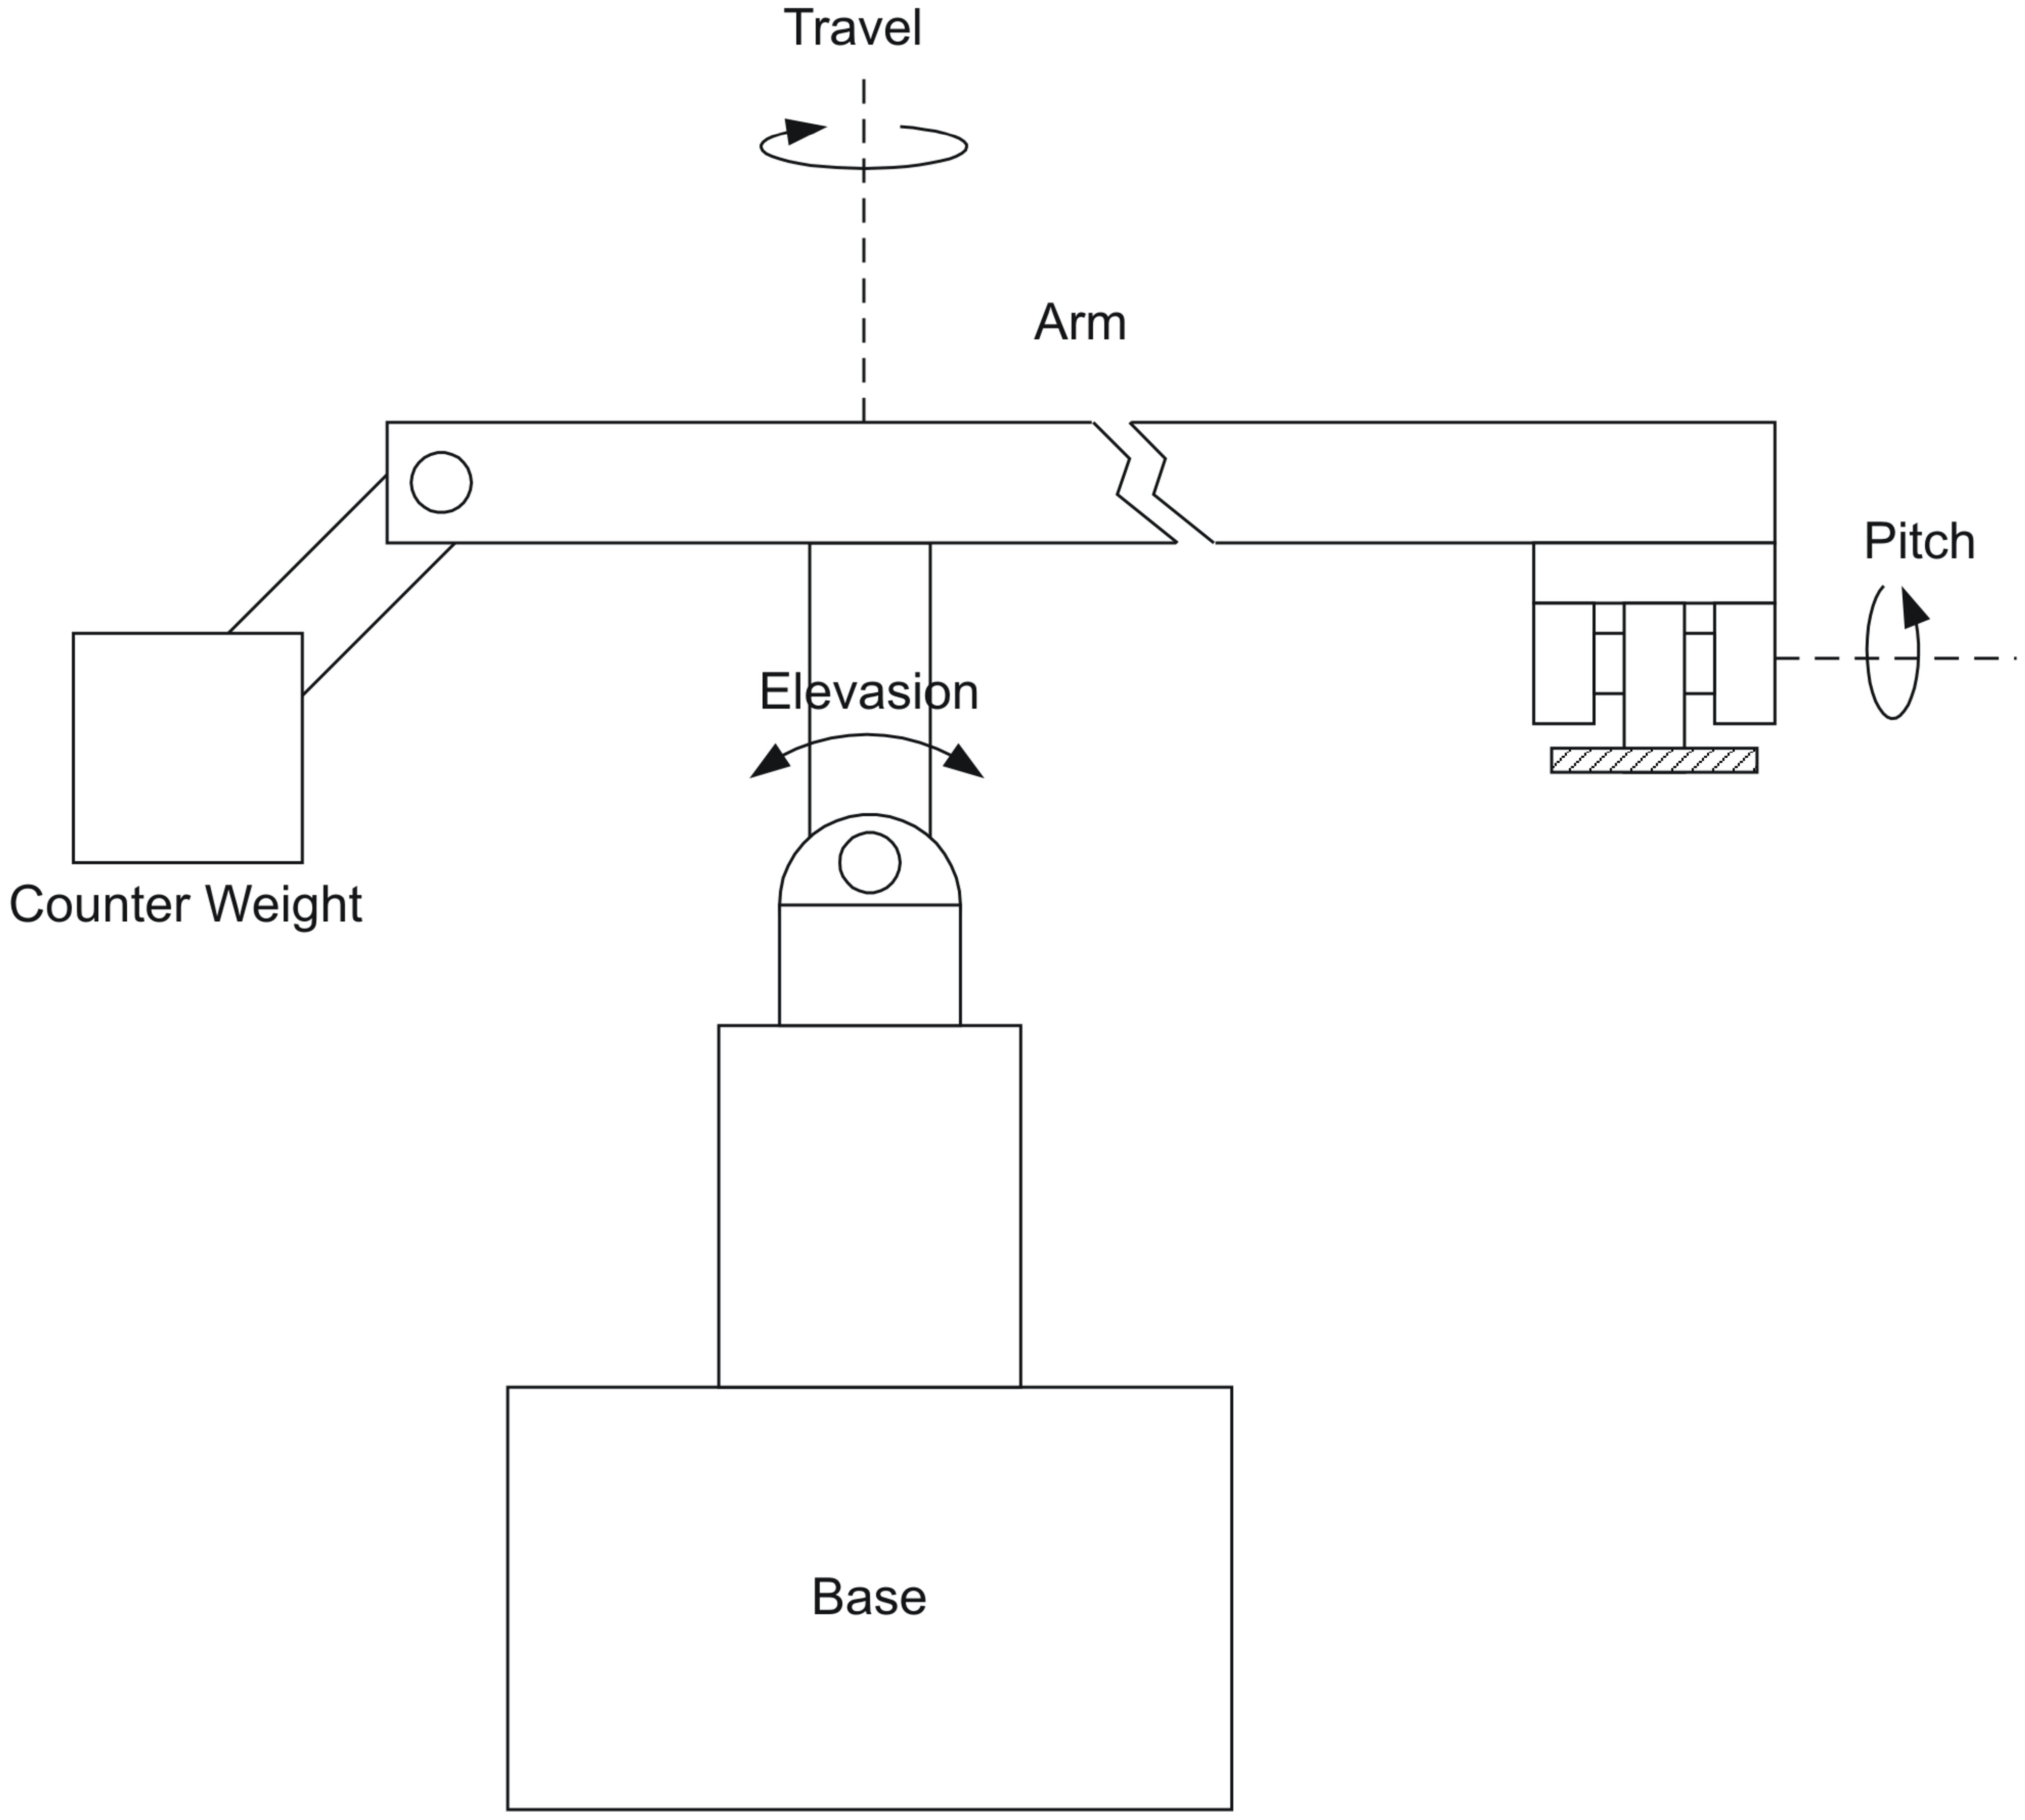
\includegraphics[width=0.5\textwidth]{model}}
\caption{Model of setup}
\label{fig:model}
\end{figure}
\noindent 
The  lab helicopter consists of a moveable arm with two rotors at one end and a counterweight at the other. The arm is attached to an elevation axis and can rotate around this. The helicopter has three degrees of freedom, travel, pitch and elevation, all of which are induced by the thrust of the two rotors. The counterweight results in the helicopter needing less thrust and also in slower dynamics. Elevation and pitch are controlled by implementing a PD controller and PID controller, respectively.
\newline
The model can be summarized by the following equations
\begin{subequations}
\label{eq:model_al}
\begin{align}
	\ddot{e} + K_{3} K_{ed} \dot{e} + K_{3} K_{ep} e &= K_{3} K_{ep} e_{c} \label{eq:model_se_al_elev} \\
	\ddot{p} + K_{1} K_{pd} \dot{p} + K_{1} K_{pp} p &= K_{1} K_{pp} p_{c} \label{eq:model_se_al_pitch} \\
	\dot{\lambda} &= r \label{eq:model_se_al_lambda} \\
	\dot{r} &= -K_{2} p \label{eq:model_se_al_r} 
\end{align}
\end{subequations}
with
\begin{subequations}
\label{eq:K}
\begin{align}
	K_{1} &= \frac{K_{f}l_{h}}{J_{p}} \label{eq:K1} \\
    K_{2} &= \frac{K_{p}l_{a}}{J_{t}} \label{eq:K2} \\
    K_{3} &= \frac{l_{a}K_{f}}{J_{e}} \label{eq:K3}
\end{align}
\end{subequations}
\newline


Where the corresponding parameters and variables are given in tables \ref{tab:parameters} and \ref{tab:variables}
\begin{table}[h]
	\centering
	\caption{Parameters and values.}
	\begin{tabular}{llll}
		\hline
		Symbol & Parameter & Value & Unit \\
		\hline
		$l_a$ & Distance from elevation axis to helicopter body & $0.63$ & \meter \\
		$l_h$ & Distance from pitch axis to motor & $0.18$ & \meter \\
		$K_f$ & Force constant motor & $0.25$ & \newton\per\volt \\
		$J_e$ & Moment of inertia for elevation & $0.83$ & \kilogram\usk\square\meter \\
		$J_t$ & Moment of inertia for travel & $0.83$ & \kilogram\usk\square\meter \\
		$J_p$ & Moment of inertia for pitch & $0.034$ & \kilogram\usk\square\meter \\
		$m_h$ & Mass of helicopter & $1.05$ & \kilogram \\
		$m_w$ & Balance weight & $1.87$ & \kilogram \\
		$m_g$ & Effective mass of the helicopter & $0.05$ & \kilogram \\
		$K_p$ & Force to lift the helicopter from the ground & $0.49$ & \newton \\
		\hline
	\end{tabular}
	\label{tab:parameters}
\end{table}

\begin{table}[h]
	\centering
	\caption{Variables.}
	\begin{tabular}{llll}
		\hline
		Symbol & Variable \\
		\hline
		$p$ & Pitch\\
		$p_c$ & Setpoint for pitch\\
		$\lambda$ & Travel\\
		$r$ & Speed of travel\\
		$r_c$ & Setpoint for speed of travel\\
		$e$ & Elevation\\
        $e_c$ & Setpoint for elevation\\
		$V_f$ & Voltage, motor in front\\
		$V_b$ & Voltage, motor in back\\
		$V_d$ & Voltage difference, $V_f - V_b$\\
        $V_s$ & Voltage sum, $V_f + V_b$\\
        $K_{pp}, K_{pd}, K_{ep}, K_{ei}, K_{ed}$ & Controller gains\\
        $T_g$ & Moment needed to keep the helicopter flying\\
		\hline
	\end{tabular}
	\label{tab:variables}
\end{table}

\begin{table}[h]
	\centering
	\caption{Controller Gains}
	\begin{tabular}{llll}
		\hline
		Gain & Value\\
        \hline
		$K_{pp}$ & 19.7653\\
		$K_{pd}$ & 2.7841\\
		$K_{ei}$ & 4.5\\
		$K_{ep}$ & 10\\
		$K_{ed}$ & 8\\
		\hline
	\end{tabular}
	\label{tab:gains}
\end{table}

\section{Repetition/Introduction to Simulink/QuaRC}\label{sec:prob1}
This part of the exercise is meant as a repetition to the helicopter model and the implementation in Simulink using QuaRC.
\begin{figure}[!h]
\centerline{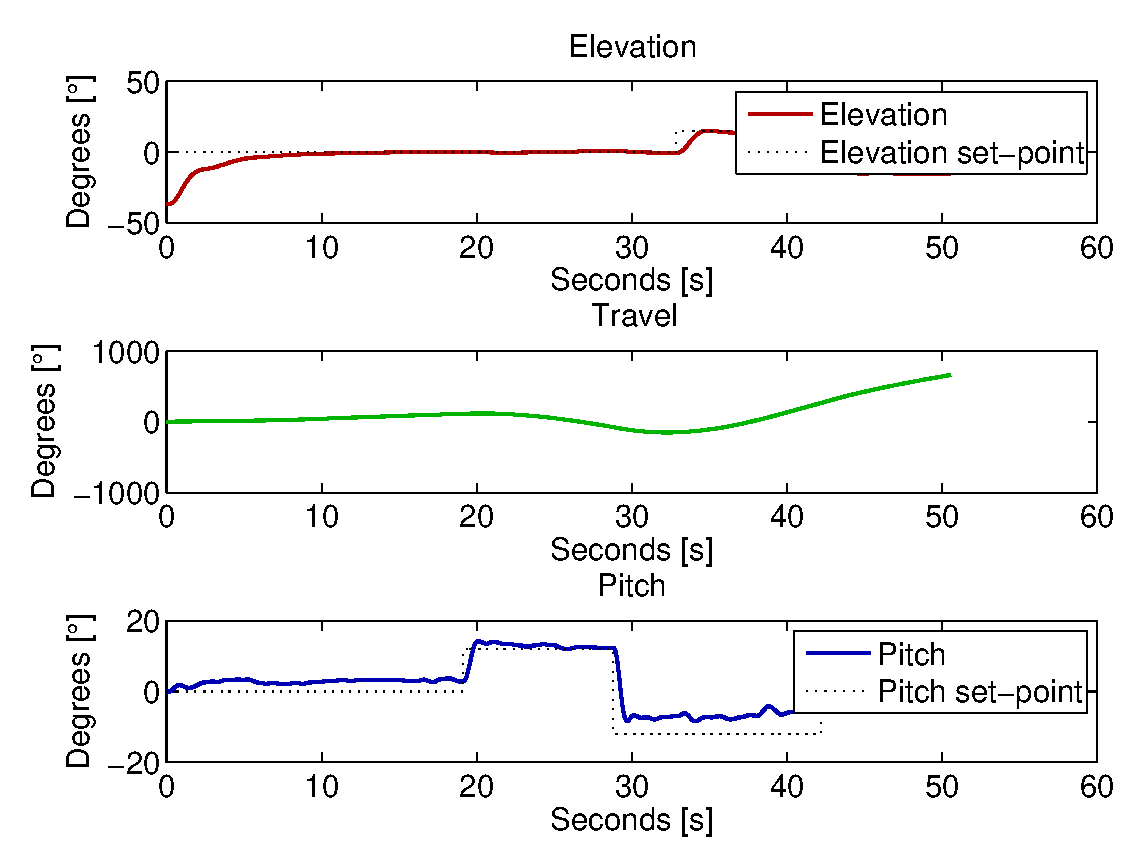
\includegraphics[width=1\textwidth]{graph1}}
\caption{Plots of test run with changing setpoints}
\label{fig:testrunplot}
\end{figure}

By adding constants to the controller inputs \verb!v_c! and \verb!p_c! (see Appendix \ref{sec:simulink:1}) we were able to change the setpoint for elevation and pitch during travel and test the functionality. As seen in Figure~\ref{fig:testrunplot} the results are satisfactory. The pitch are unable to reach setpoint when combined with increased elevation, due to the dynamics of the system\textcolor{red}{??????}

\subsection{Results and discussion}
This part of the problem verified that the helicopter was functioning properly. However, the helicopter was drifting slightly. This is probably due to the fact that the motors do not have individual motor constants - they are treated as identical with the same motor constant. \textcolor{red}{ha med noe om unoeyaktig modell?}

\section{Optimal Control of Pitch/Travel without Feedback}\label{sec:prob2}

In this section the optimal state trajectory, $\mathbf{x}^*$, and the optimal input sequence, $u^*$, for the helicopter are computed. State feedback is not implemented, hence the controller does not compensate for undesired deviations from the optimal trajectories. The elevation is disregarded in this part, i. e. $e = 0$. The objective is to calculate an optimal trajectory that moves the helicopter from an initial state, $\lambda_0 = 180^{\circ}$, to a final state, $\lambda_f = 0^{\circ}$.

\begin{figure}[!h]
    \begin{minipage}{\textwidth}
\centerline{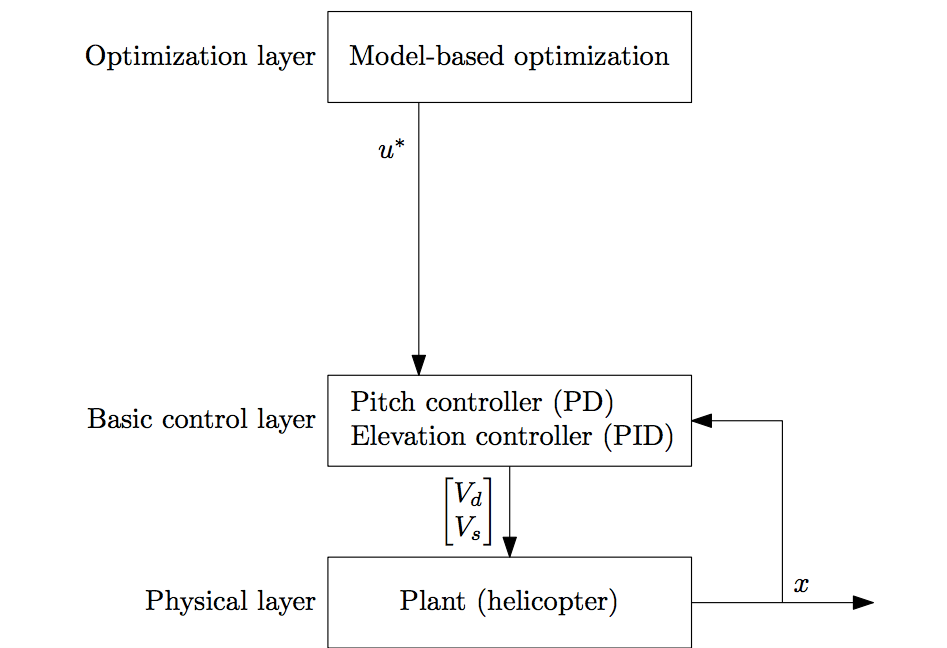
\includegraphics[width=1.0\textwidth]{10_2bilde}}
    \end{minipage}
    \caption{Control hierarchy for section 4}
	\label{fig:10_2bilde}
\end{figure}

\subsection{Continuous-time model}
The model can be written on continuous time state space form
\begin{equation}
    \mathbf{\dot{x}} = \mathbf{A_cx} + \mathbf{B_c} u
    \label{eq:axbu}
\end{equation}
with states $\mathbf{x} = \begin{bmatrix} \lambda & r & p & \dot{p} \end{bmatrix}^\top$, and input $u = p_c$. Rearranging the summarized equations (\ref{eq:model_al}), the model can be written
\begin{equation}
	\begin{bmatrix}
    \dot{\lambda}\\ \dot{r} \\ \dot{p} \\ \ddot{p}
    \end{bmatrix}
    = \underbrace{\begin{bmatrix} 0 & 1 & 0 & 0 \\ 0 & 0 & -K_2 & 0 \\ 0 & 0 & 0 & 1 \\ 0 & 0 & -K_1K_{pp} & -K_1K_{pd} \end{bmatrix}}_{\mathbf{A_{c}}}
    \begin{bmatrix} \lambda \\ r\\ p\\ \dot{p}
    \end{bmatrix}
    +\underbrace{\begin{bmatrix}0 \\ 0 \\ 0 \\K_1K_{pp} \end{bmatrix}}_\mathbf{{B_{c}}}
    p_{c}
\end{equation}
with $K1$, $K2$, $K3$ as in \eqref{eq:K}, and the controller gains $K_{pp}$ and $K_{pd}$ takes the values from table \eqref{tab:gains}.
\newline

\textcolor{red}{What are we modeling here? Is it just the helicopter?}
This model uses the four states, travel, travel rate, pitch and pitch rate with the desired pitch angle as the only input. Elevation and elevation rate is disregarded in this model. The voltage sum $V_s = V_f + V_b$ controls the elevation of the helicopter. As seen in figure \eqref{fig:10_2bilde} and the Simulink diagram in Appendix \ref{sec:simulink:1}, the basic control layer incorporates two controllers, a PD-controller for pitch and a PID controller for elevation. The reference for the elevation controller is constant. This implies that the four states in this section can be controlled independently of the elevation and elevation rate.

The decoupling of the states results in a simpler model for the helicopter. However, this further reduces the accuracy of the model.

\subsection{Discrete-time model}
The system is discretized using the forward Euler method \footnote{Egeland and Gravdahl (2003)}.

\begin{equation}
    \mathbf{\dot{x}} \approx \frac{\mathbf{x_{k+1}} - \mathbf{x_k}}{h}
    \label{eq:forwardEuler}
\end{equation}
Where $h$ is the time step between each sampling $k$. Combining \eqref{eq:forwardEuler} and \eqref{eq:axbu}

\begin{align}
\label{eq:discretization}
    	\mathbf{x_{k+1}} &= h\mathbf{A_{c}x_{k}}+h\mathbf{B_{c}}u_{k}+\mathbf{x_k}\\
        &=(\mathbf{I} + h\mathbf{A_c}) \mathbf{x_k} + h\mathbf{B_c} u_k \nonumber \\
        &=\mathbf{A x_k} + \mathbf{B} u_k \nonumber
\end{align}
where
\begin{equation}
    \mathbf{A} = \mathbf{I} + h\mathbf{A_c}
    \qquad\text{and}\qquad
    \mathbf{B} = h\mathbf{B_c}
\end{equation}
The step size is set to $h = 0.25$ seconds for the the entire duration of this report.
The resulting system matrices on discrete time state space form are
\begin{equation}
    \mathbf{A} = \begin{bmatrix} 1 & h & 0 & 0 \\ 0 & 1 & -hK_2 & 0 \\ 0 & 0 & 1 & h \\ 0 & 0 & -K_1K_{pp} & 1-hK_1K_{pd} \end{bmatrix}
    \qquad\text{and}\qquad
    \mathbf{B} = \begin{bmatrix}0 \\ 0 \\ 0 \\hK_1K_{pp} \end{bmatrix}
\end{equation}

\subsection{Optimal trajectory}
In this section the following cost function is minimized
\begin{equation}
\phi=\sum_{i=1}^{N}(\lambda_i-\lambda_f)^2+qp_{ci}^2,\;\; q\geq0
\label{costFunction1}
\end{equation}
with the given linear constraint
\begin{equation}
\mid{P_k}\mid\leq\frac{30\pi}{180},\;\;   k\in\{1,...,N\}
\end{equation}
which restricts the pitch and pitch set point to 30 degrees. The objective in this section is to control the helicopter from the initial state, $x_0=\begin{bmatrix}\lambda_0 & 0 & 0 & 0 \end{bmatrix}^\top$, to the desired state, $x_f=\begin{bmatrix}\lambda_f & 0 & 0 & 0 \end{bmatrix}^\top$, where $\lambda_0=180^{\circ}$ and $\lambda_f=0^{\circ}$. In this case the manipulated variable, $u=p_{ci}$, is weighted by a factor q. The cost function given in \eqref{costFunction1} is clearly a QP problem, and is written on standard form
\begin{equation}
\label{eq:QP1}
\phi = \frac{1}{2}\sum\limits_{i=0}^{N-1} \{ \mathbf{x}_{i+1}^\top \mathbf{Q} \mathbf{x}_{i+1} + u_i R u_i\}
\end{equation}\\
where
\begin{equation}
\label{eq:Q1}
Q = 2 \cdot \text{diag}
\begin{bmatrix}1 & 0 & 0 & 0\end{bmatrix} \text{,} \quad R = 2 \cdot q
\end{equation}
Furthermore, the system can be written on the following form
\begin{equation}
\begin{aligned}
	& \underset{z}{\text{min}}
	& & \mathbf{z}^\top \mathbf{G z} \\
	& \text{subject to}
	& & \mathbf{A}_{eq} \mathbf{z} = \mathbf{B}_{eq}
	\end{aligned}
\end{equation}
where the optimization variable, $z$, includes the state vector, $x$, and the input sequence, $u$. 
\begin{equation}
\mathbf{z} = \begin{bmatrix} \mathbf{x}_1^\top, & \ldots & ,\mathbf{x}_N^\top, & u_0^\top, & \ldots & ,u_{N-1}^\top \end{bmatrix}^\top \in  \mathbb{R}^{500 \times 1}
\end{equation}
The weighting matrix $\mathbf{G}$ and the constraint matrices $\mathbf{A_{eq}}$ and $\mathbf{B_{eq}}$ are written as follows
\begin{equation}
\mathbf{G} = \begin{bmatrix}
\mathbf{Q} 	& \mathbf{0}& \cdots & \cdots & \cdots & \mathbf{0}\\
\mathbf{0} 	& \ddots 	& \ddots 	& 		  & 	   & \vdots \\
\vdots 		& \ddots 	& \mathbf{Q} & \ddots & 	& \vdots\\
\vdots 		&  			& \ddots 	& R 	& \ddots & \vdots\\
\vdots 		& 			& & \ddots 	& \ddots & \mathbf{0}\\
\mathbf{0} 	& \cdots 	& \cdots 	& \cdots & \mathbf{0} & R
\end{bmatrix} \in  \mathbb{R}^{500 \times 500}
\end{equation}

\begin{equation}
\label{eq:Aeq}
\mathbf{A}_{eq} = \begin{bmatrix}
\mathbf{I} & \mathbf{0} & \cdots & \cdots & \mathbf{0} & - \mathbf{B} & \mathbf{0} & \cdots & \cdots & \mathbf{0}\\
-\mathbf{A} & \mathbf{I} & & & \vdots & \mathbf{0} & \ddots & \ddots & & \vdots\\
\mathbf{0} & \ddots & \ddots & & \vdots & \vdots & \ddots & \ddots & \ddots & \vdots\\
\vdots & & \ddots & \ddots & \mathbf{0} & \vdots & & \ddots & \ddots & \vdots \\
\mathbf{0} & \cdots & \mathbf{0} & -\mathbf{A}  & \mathbf{I} & \mathbf{0} & \cdots & \cdots & \mathbf{0} & -\mathbf{B}
\end{bmatrix} \in  \mathbb{R}^{400 \times 500}
\end{equation}

\begin{equation}
\label{eq:Beq}
\mathbf{B}_{eq} = \begin{bmatrix}\mathbf{A x_0} \\ \mathbf{0}\\ \vdots \\ \mathbf{0} \end{bmatrix} \in \mathbb{R}^{400 \times 1}
\end{equation}\\

The optimization problem was solved in matlab using the built-in function \verb!quadprog! over a time horizon $N = 100$. With a time step $h = 0.25$ seconds, the helicopter would run for 25 seconds. In addition, the helicopter was kept stable at the initial state by adding 5 seconds of zeros before and after the optimal input sequence. The optimal input sequence was fed into the pitch controller in the basic control layer.\\

Optimal trajectories were computed for different values of $q$, without using state feedback. When the weighting scalar $q$ was changed, the manipulated variable, $p_c$, was punished in alternating degree.
Three different values were implemented for $q$, 0.1, 1 and 10. The Optimal trajectories for the different values of q are shown in Figure \ref{fig:q_0.1_1_10}.\\
The optimal trajectories for the manipulated variable and the pitch coincide for the different values of $q$. It is worth noticing that the trajectory for the manipulated variable is step wise continuous, while the trajectory for pitch is smooth.
From Figure \ref{fig:q_0.1_1_10} it is observed that the controller penalizes the control input harder for greater values of $q$, and less for smaller values of $q$, i. e. greater changes for the control input are allowed for $q=0.1$ than $q=1$ and $q=10$.\\

The cost function in \eqref{costFunction1} takes travel, the pitch set point and weighting of them into account. The term $(\lambda_i-\lambda_f)^2$ is the deviation from the final travel value at each indices. When steering the helicopter to the desired position, $\lambda=\lambda_f$, unwanted effects could arise. The cost function does not take travel rate into account, which can lead to that the helicopter does not stop at the desired position when the optimal sequence is done. 

\begin{figure}[!h]
    \begin{minipage}{\textwidth}
\centerline{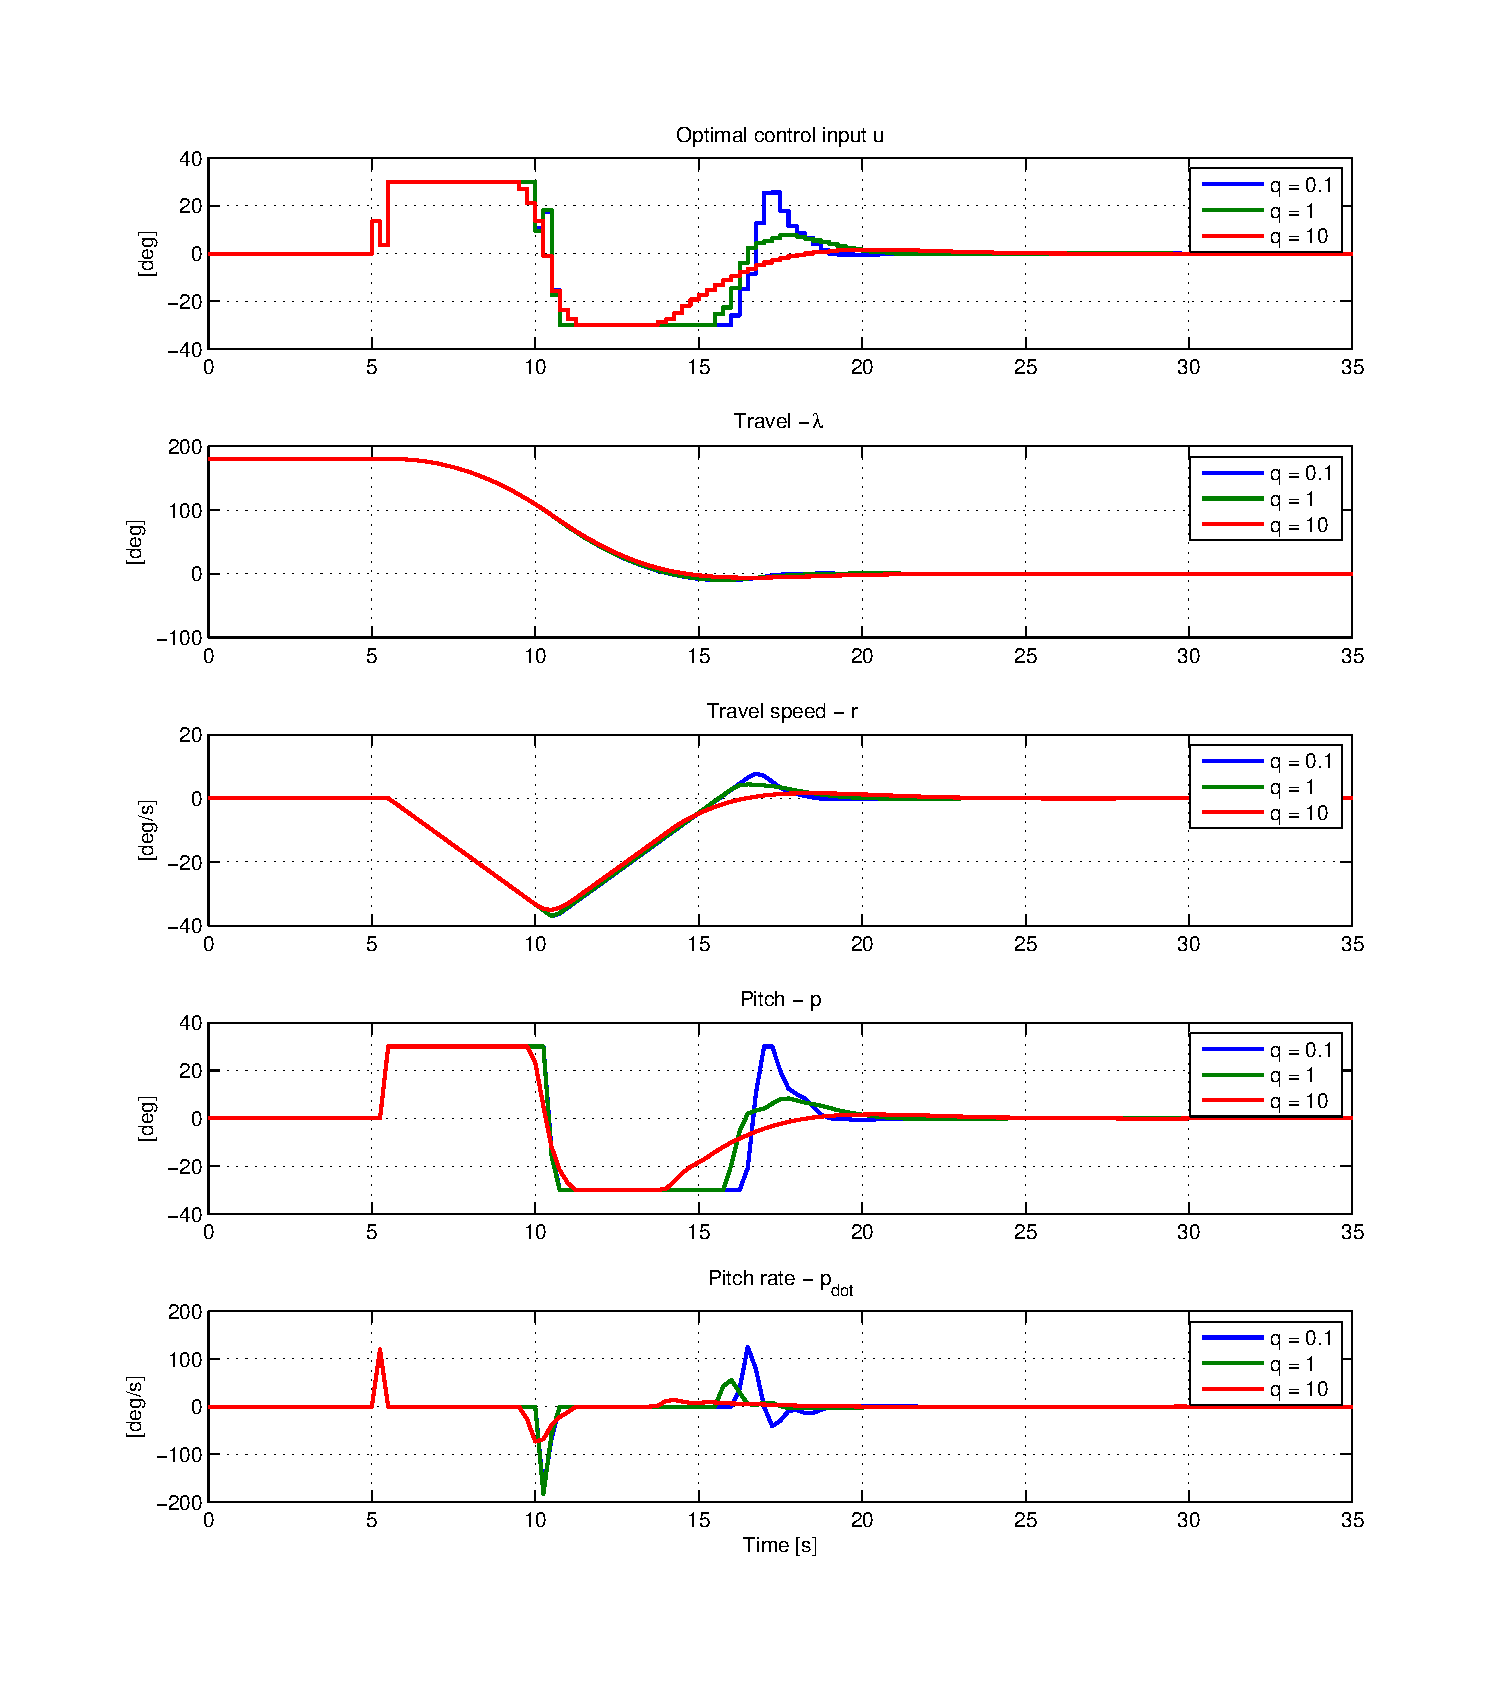
\includegraphics[width=1.3\textwidth]{optreg_10_2_3_Comparison_of_q_}}
    \end{minipage}
    \caption{Optimal trajectories for different values of q without state feedback}
	\label{fig:q_0.1_1_10}
\end{figure}


\newpage
\subsection{Implementation}
% q = 0.1
\begin{figure}[!h]
    \begin{minipage}{\textwidth}
  \centerline{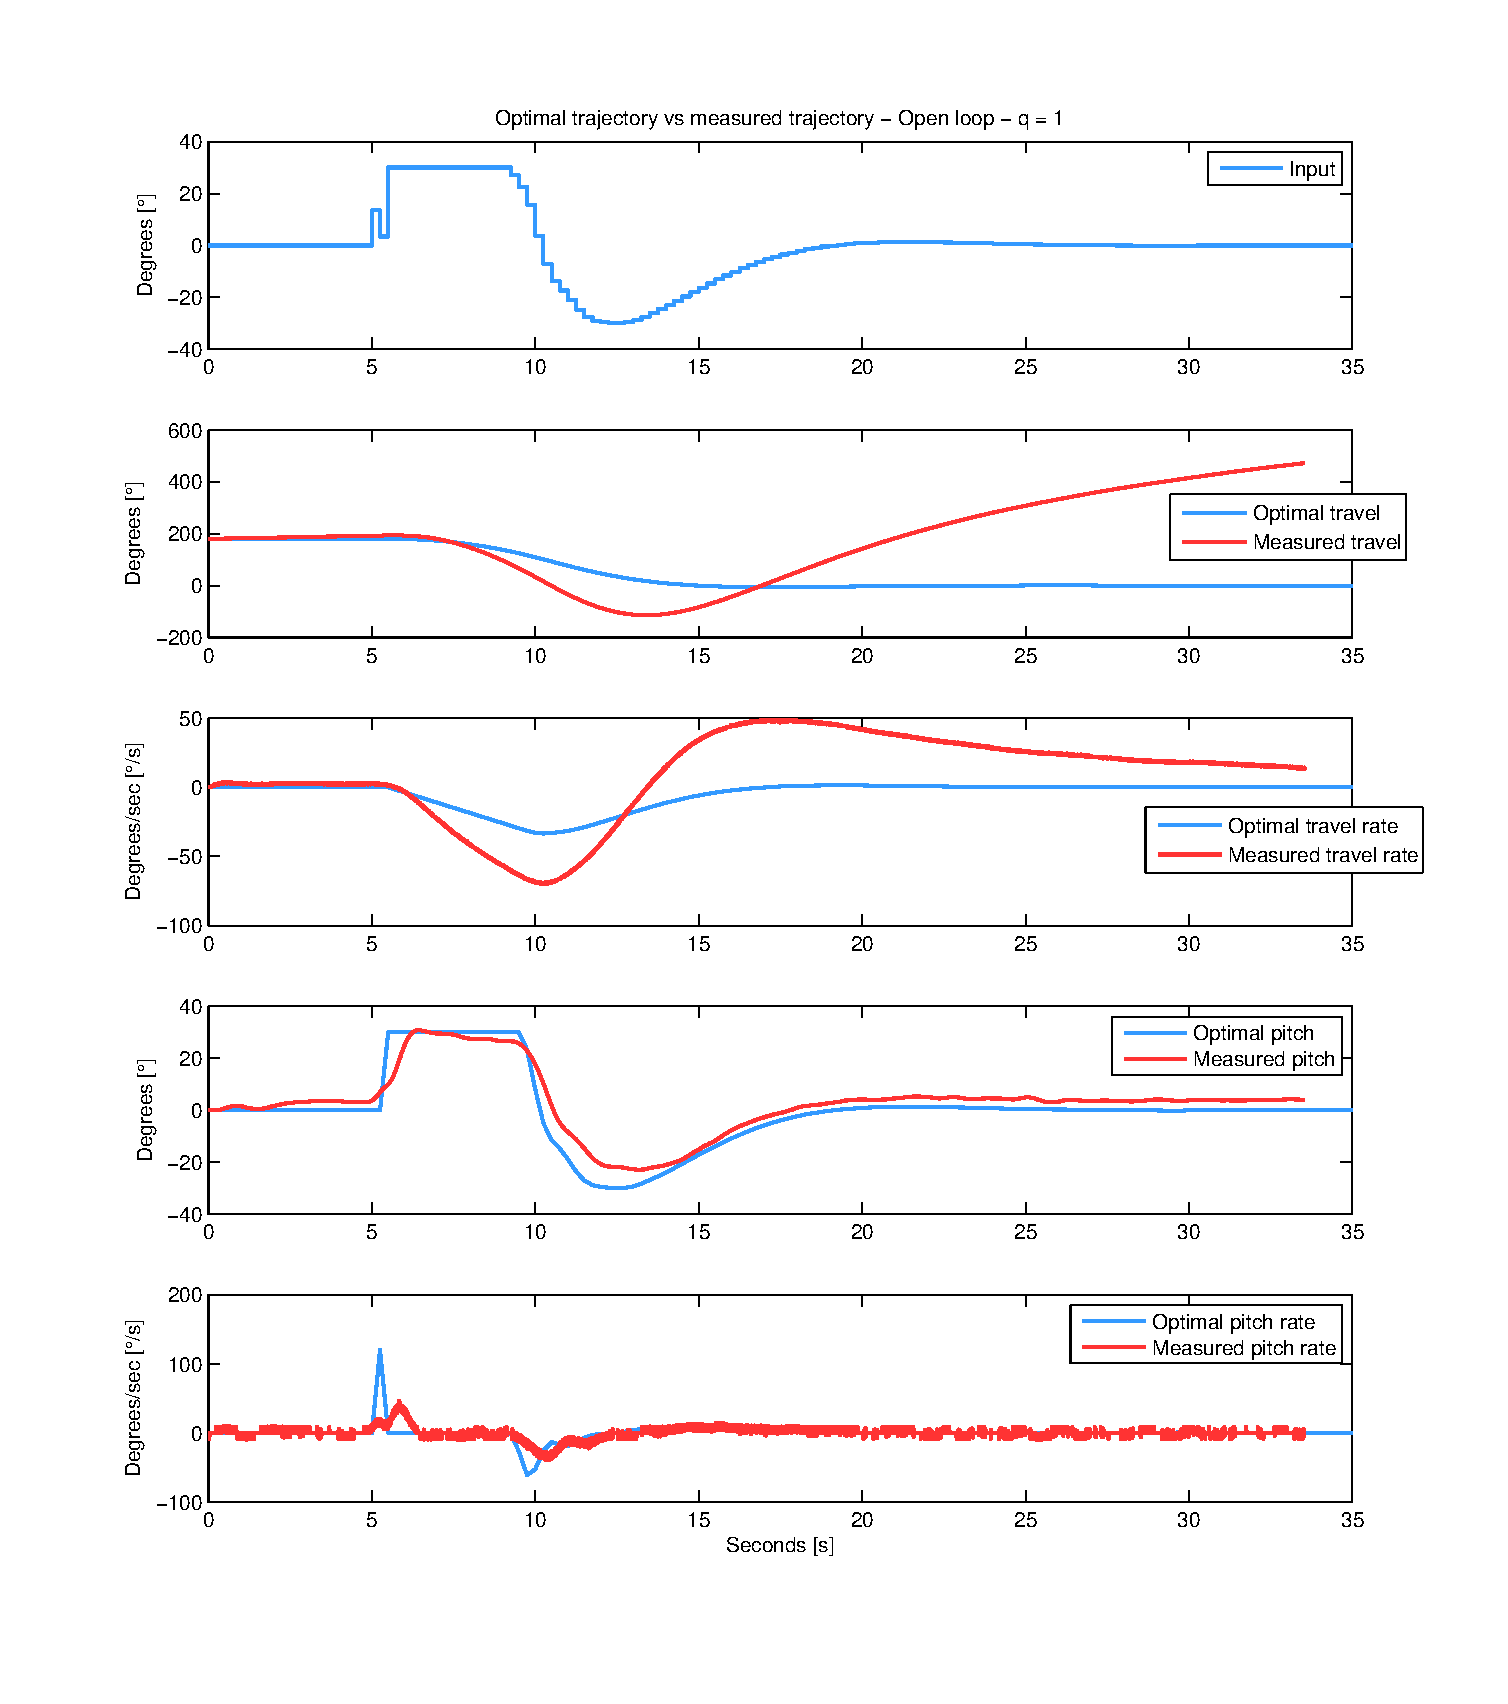
\includegraphics[width=1.3\textwidth]{opg2_compare_q1}}
	\caption{Comparison of measured and optimal states with q = 1}
    \end{minipage}
	\label{fig:q01}
\end{figure}
\newpage
\subsection{Results and discussion}
As clearly seen in figure \ref{fig:q01}, the helicopter failed to reach the planned final state for $q = 1$, even though pitch and pitch rate coincides well with the optimal trajectory. Trying with different values for $q$ did not improve the results.

Unlike pitch, travel is not controlled by a designated controller in the basic control layer. In addition, modeling errors, linearization errors and disturbances makes it hard for the helicopter to follow the optimal trajectory.

It is not realistic to construct a perfect model, and therefore, feedback is necessary to control the helicopter in a satisfactory way.

\section{Optimal Control of Pitch/Travel with Feedback (LQ)}\label{sec:prob3}

Feedback for the system is introduced by adding a correcting term to the optimal input.

In this section, feedback is introduced to the optimal controller to correct for deviations from the optimal trajectory caused by modeling errors. For this purpose, an LQ controller is suitable as the controller minimizes a quadratic criteria for a linear model. We also discuss if Model Predictive Control would be a good alternative to LQR.

\begin{figure}[!h]
    \begin{minipage}{\textwidth}
\centerline{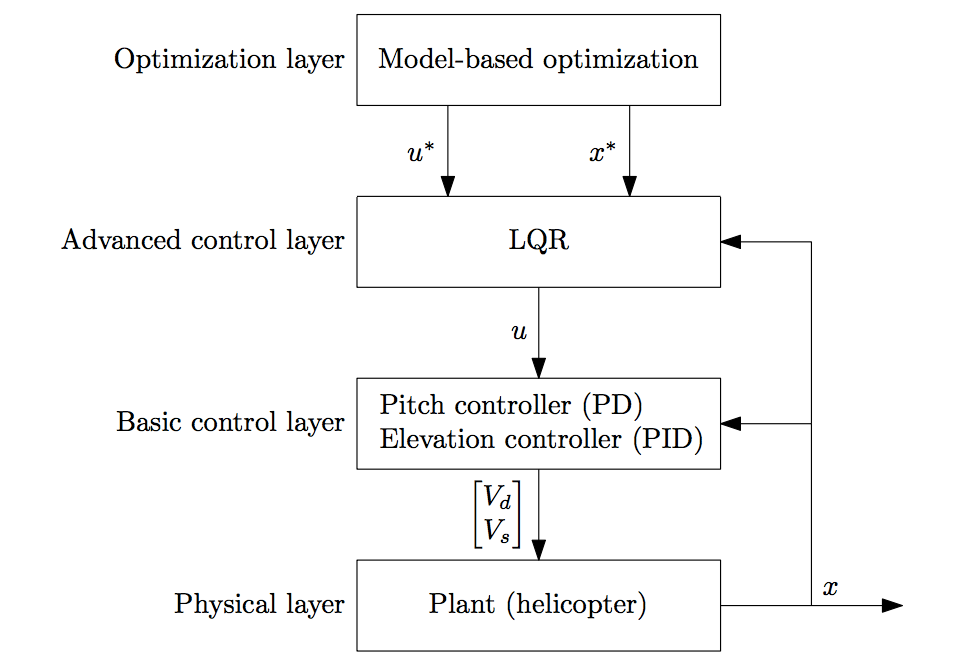
\includegraphics[width=1.0\textwidth]{10_3bilde}}
    \end{minipage}
    \caption{Control hierarchy for section 5}
	\label{fig:10_3bilde}
\end{figure}


\subsection{Linear Quadratic (LQ) Controller}
We introduce a feedback control law
\begin{equation}
    u_k = u_k^* - \mathbf{K}^T(\mathbf{x}_k - \mathbf{x}_k^*)
\end{equation}
Where $u_k^*$ is the optimal input sequence and $x_k^*$ is the optimal trajectory. This can be written as
\begin{equation}
\label{eq:delta_uk}
\Delta u_k = -\mathbf{K}^\top \Delta \mathbf{x}_k
\end{equation}
where
\begin{equation}
\Delta u_k = u_k - u^*\quad \text{and} \qquad \Delta \mathbf{x}_k = \mathbf{x}_k - \mathbf{x}^*_k
\end{equation}
are deviations from the optimal trajectory.
The optimal controller gain $\mathbf{K}$ is found by minimizing 
\begin{equation}
    \label{eq:lqr_cost}
    J = \sum_{i=0}^\infty {\Delta \mathbf{x}_{i+1}^\top \mathbf{Q} \Delta \mathbf{x}_{i+1} + \Delta u_{i}^\top R\Delta u_{i}}, \;\;\; \mathbf{Q} \geq 0, \; R \geq 0
\end{equation}
where $\Delta u_i = -\mathbf{K} \Delta \mathbf{x}_{i} (i eller i+1?)$ subject to the linear model $\Delta \mathbf{x}_{i+1} = \mathbf{A}\Delta \mathbf{x}_i + \mathbf{B}\Delta u_i$.

This is done with the MATLAB function \verb!dlqr!, which solves \eqref{eq:lqr_cost} where:

\begin{equation}
	\label{eq_ricattiK}
    \mathbf{K} =     
\end{equation}

$\mathbf{Q} \succeq 0$ and $\mathbf{R} \succ 0$ are weighting matrices that can be chosen to penalize individual deviations in states or input.


The state weighing matrix $\mathbf{Q}$ is chosen as diagonal matrix, and $R$ as a constant. $\mathbf{Q}$ was then tuned by increasing or decreasing the weights along the diagonal, to fit our purpose of having a travel trajectory as close as
possible to the optimal trajectory, but without too much oscillations in pitch. The following $\mathbf{Q}$ and $R$ yielded a satisfying result.
\begin{equation}
    \mathbf{Q} = \begin{bmatrix} 100 & 0 & 0 & 0 \\ 0 & 50 & 0 & 0 \\ 0 & 0 & 0.01 & 0 \\ 0 & 0 & 0 & 3 \end{bmatrix}
    \qquad\text{and}\qquad
    R = 2
\end{equation}

 For our choice of these, the controller gain was found to be
\begin{equation}
\mathbf{K} = \begin{bmatrix} ? & ? & ? & ?\end{bmatrix}^\top
\end{equation}

\subsection{Implementation of feedback}
The block diagram structure of the helicopter with feedback can be seen in the Simulink diagram in Appendix \ref{sec:simulink:3}.

\begin{figure}[!h]
    \begin{minipage}{\textwidth}
 \centerline{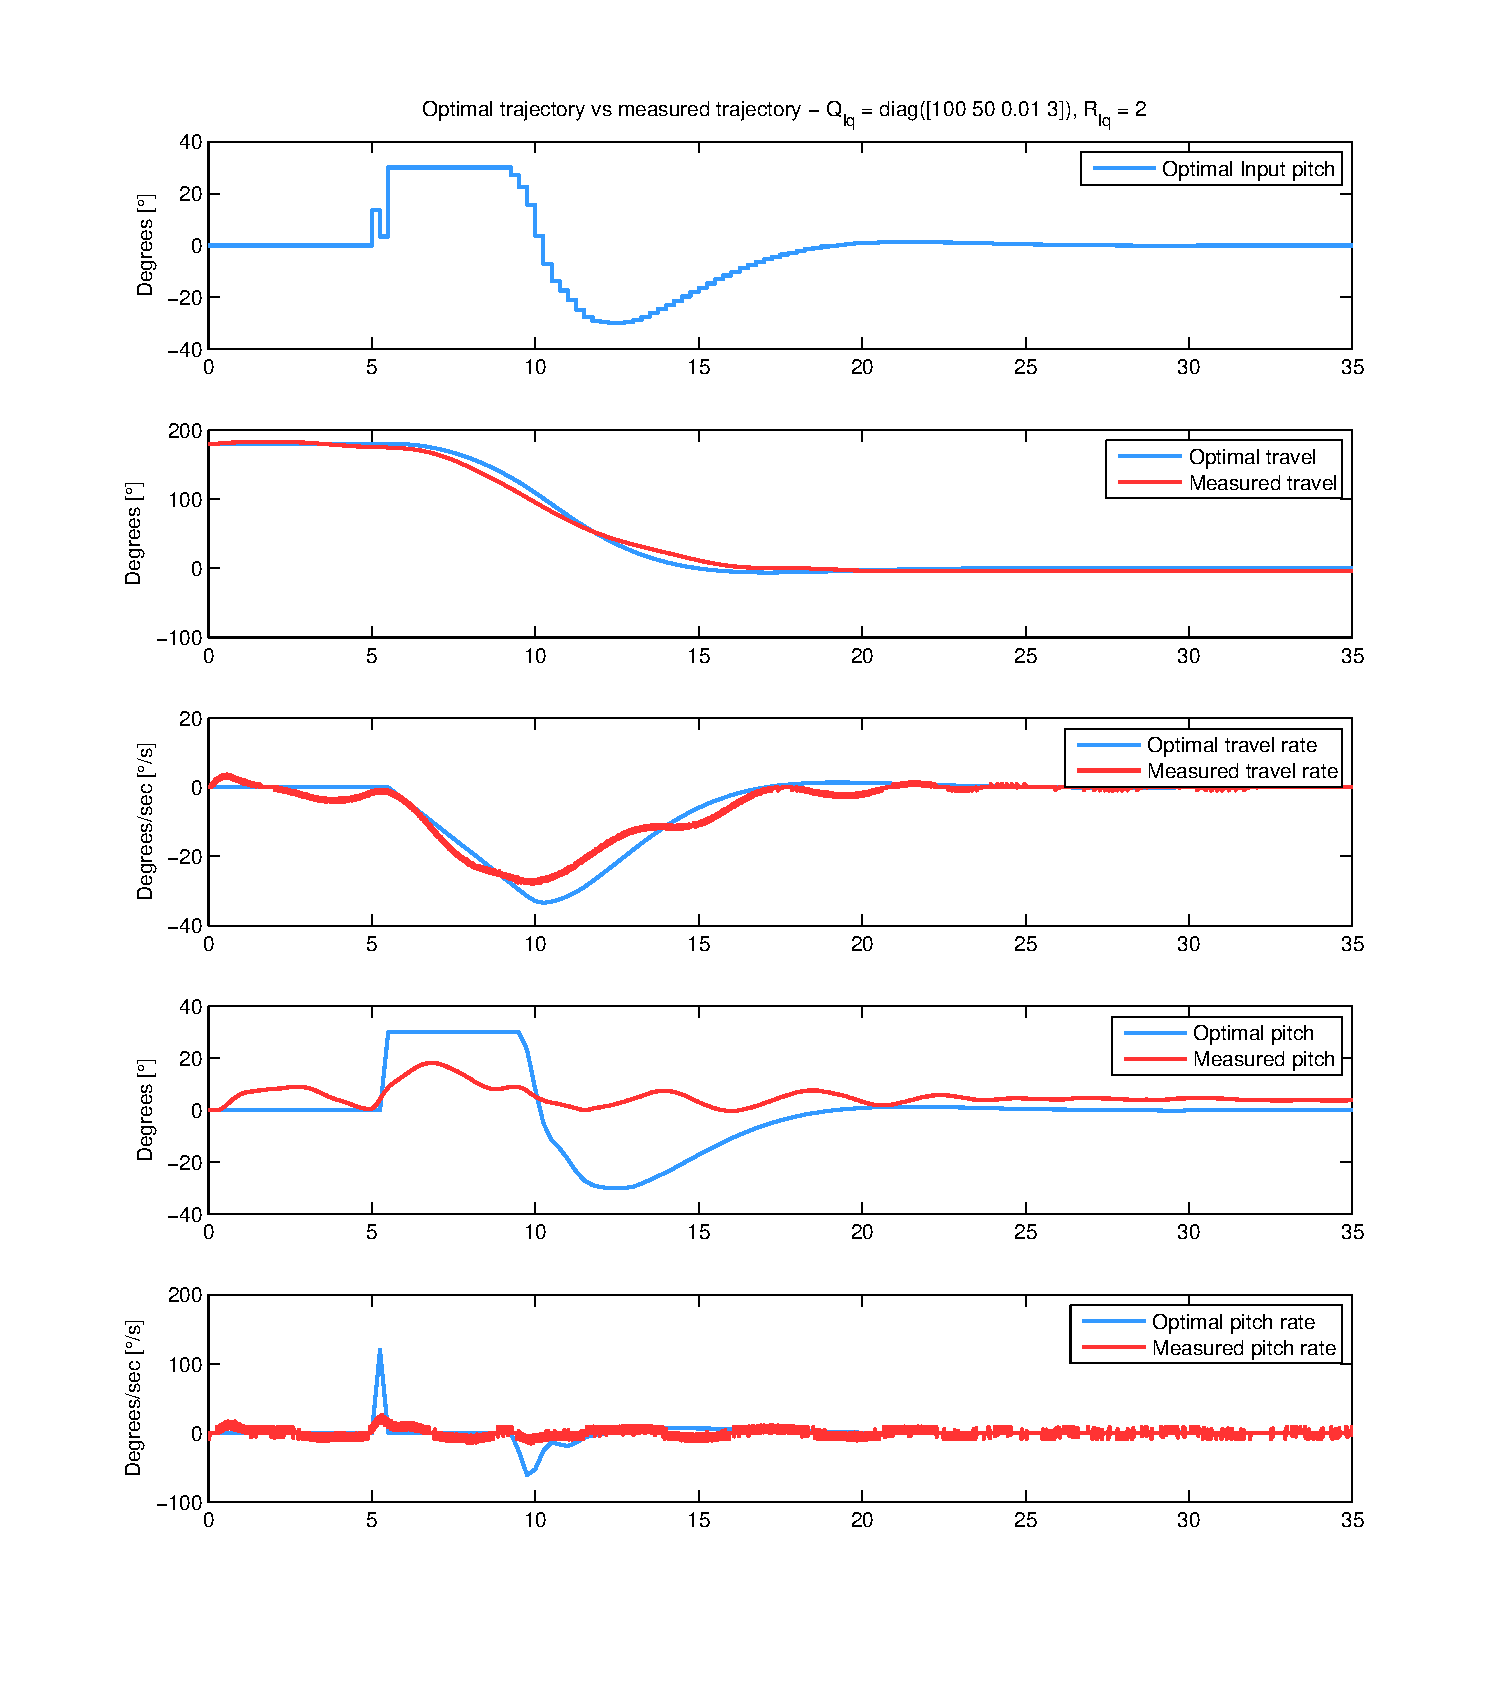
\includegraphics[width=1.3\textwidth]{optreg_10_3_2}}
	\caption{Optimal and measured travel and pitch trajectories with optimal input sequence using feedback}
    \end{minipage}
	\label{fig:10_3_2}
\end{figure}

\subsection{Results and discussion}
The results seen in figure \ref{fig:10_3_2} shows that the helicopter follows the optimal travel trajectory, however, the optimal and measured pitch do not coincide. hvorfor det?


\subsection{Model Predictive control (MPC)}
An MPC controller could be realized by calculating a new optimal trajectory at each time step. The first time step of each calculated optimal input sequence should then be used as the input $u_t$ for that time step. The advantage of using MPC instead of LQR is that constraints may be applied to the system. The MPC controller might result in less demanding input for a given trajectory, and does also provide implicit feedback, which is important for a control system with modelling errors and disturbances. The main disadvantage of using MPC is that it takes heavy calculations, which takes a lot of time. The calculations has to be done during run time, which may be bad if the control system is slower than the helicopter. The control hierarchy with MPC would have replaced the Advanced control layer by the Optimization layer, leading to one less layer in the hierarchy in Figure \ref{fig:10_3bilde}.

\newpage


\section{Optimal Control of Pitch/Travel and Elevation with and without Feedback}\label{sec:prob4}
\subsection{Continous-time model}
In this section elevation and elevation rate are included in the state vector, since the helicopter must avoid a restriction along its path. The state vector is written as

\begin{equation} 
	\mathbf{x} =
\begin{bmatrix}
	\lambda & r & p & \dot{p} & e & \dot{e}
\end{bmatrix}^T
\end{equation}
The continuous state-space model of the system is

\begin{equation}
    \mathbf{\dot{x}} = \mathbf{A_cx} + \mathbf{B_c}\mathbf{u}
    \label{eq:axbu2}
\end{equation}
Where the state matrix, $A_c$, and the input matrix, $B_c$, are calculated as

\begin{equation}
    \mathbf{A_c} = \begin{bmatrix} 0 & 1 & 0 & 0 & 0 & 0 \\ 0 & 0 & -K_2 & 0 & 0 & 0  \\ 0 & 0 & 0 & 1 & 0 & 0 \\ 0 & 0 & -K_1K_{pp} & -K_1K_{pd} & 0 & 0 \\ 0 & 0 & 0 & 0 & 0 & 1 \\ 0 & 0 & 0 & 0 & -K_{3}K_{ep} & -K_{3}K_{ed}
\end{bmatrix}
\end{equation}
\begin{equation}
    \mathbf{B_c} = \begin{bmatrix}0 & 0 \\ 0 & 0 \\ 0 & 0 \\ K_1K_{pp} & 0 \\ 0 & 0 \\ 0 &  K_{3}K_{ep} \end{bmatrix}
    \label{eq:sselev}
\end{equation}

\subsection{Discrete-time model}
The system is linearized using the forward Euler method. 

\begin{equation}
    \mathbf{\dot{x}_k} \approx \frac{\mathbf{x_{k+1}} - \mathbf{x_k}}{h}
\end{equation}
Substituting the state-space model \eqref{eq:axbu}, we obtain
\begin{equation}
    \mathbf{x_{k+1}} \approx h\mathbf{A_{c}}\mathbf{x_{k}}+h\mathbf{B_{c}}\mathbf{u_{k}+\mathbf{x_{k}}}
    \label{discrete}
\end{equation}
which is the same as
\begin{equation}
    \mathbf{x_{k+1}} \approx (\mathbf{I} + h\mathbf{A_c}) \mathbf{x_k} + h\mathbf{B_c} \mathbf{u_k}
    \label{disc}
\end{equation}
from \eqref{disc}, we see that
\begin{equation}
    \mathbf{A} = \mathbf{I} + h\mathbf{A_c}
    \qquad\text{and}\qquad
    \mathbf{B} = h\mathbf{B_c}
\end{equation}
where $h$ is the step size and forward difference timestep of the discretized system.
Written in state-space form: 
\begin{equation}
    \mathbf{A_c} = \begin{bmatrix} 
    1 & h & 0 & 0 & 0 & 0 \\ 
    0 & 1 & -hK_2 & 0 & 0 & 0 \\ 
    0 & 0 & 1 & h & 0 & 0 \\ 
    0 & 0 & -hK_1K_{pp} & 1-hK_1K_{pd} & 0 & 0 \\ 
    0 & 0 & 0 & 0 & 1 & h \\ 
    0 & 0 & 0 & 0 & -hK_{3}K_{ep} & 1-hK_{3}K_{ed}
\end{bmatrix}
\end{equation}
\begin{equation}
    \mathbf{B_c} = \begin{bmatrix}0 & 0 \\ 0 & 0 \\ 0 & 0 \\ hK_1K_{pp} & 0 \\ 0 & 0 \\ 0 &  hK_{3}K_{ep} \end{bmatrix}
    \label{eq:ssdisc}
\end{equation}



\subsection{Without feedback}
\begin{equation}
\label{eq:min104}
\phi = \sum_{i=1}^N(\lambda_i - \lambda_f)^2 + q_1p^2_{ci}+q_2e^2_{ci}
\end{equation}
\begin{equation}
c(x_k)= \alpha e^(-\beta(\lambda_k-\lambda_t)^2) - e_k \leq 0
\end{equation}
\subsection{With feedback}
\subsection{Decoupled states}
\subsection{Adding more constraints}
\subsection{Results and Discussion}

\section{Discussion}\label{sec:discussion}


\section{Conclusion}\label{sec:conclusion}


\appendix
\section{MATLAB Code}\label{sec:matlab}
\subsection{Task 10.2}

%% KODE til 10.2

\sloppy
\definecolor{lightgray}{gray}{0.5}
\setlength{\parindent}{0pt}

\subsection*{Init}

\begin{verbatim}
run('init01');
\end{verbatim}



\begin{verbatim}
dt = 0.25;  % sampling time
wait = 5; % Waiting time
\end{verbatim}


\subsection*{Discrete model - system matrices}

\begin{verbatim}
A = [1 dt 0 0; 0 1 -K_2*dt 0; 0 0 1 dt; 0 0 -K_1*K_pp*dt 1-K_1*K_pd*dt];
B = [0; 0; 0; K_1*K_pp];

for i = 1:3
\end{verbatim}


\subsection*{Weighting matrices}

\begin{verbatim}
if i == 1
    q = 0.1;
elseif i == 2
    q = 1;
else
    q = 10;
end
Q = 2*[1 0 0 0; 0 0 0 0; 0 0 0 0; 0 0 0 0];
R = 2*q;
\end{verbatim}


\subsection*{Initial}

\begin{verbatim}
N = 100;        %Horizon
nx = size(A,2); % Number of states
nu = size(B,2); % Number of inputs

lambda_0 = pi;
lambda_f = 0;

x0 = [lambda_0 0 0 0]';
xf = [lambda_f 0 0 0]';

z = zeros(N*(nx+nu),1);
z0 = z;
z0(1,1) = lambda_0;
\end{verbatim}


\subsection*{Constraints}

\begin{par}
G matrix
\end{par} \vspace{1em}
\begin{verbatim}
G1 = kron(eye(N),Q); % Upper left block of G
G2 = kron(eye(N),R); % Lower right block of G
G = blkdiag(G1,G2); % Complete G-matrix


%Aeq matrix
Aeq1 = kron(eye(N),eye(nx)); % left side: 1s on diagonal
Aeq2 = kron(diag(ones((N-1),1),-1), -A); %left side: -A on diagonal shifted down on step
Aeq3 = kron(eye(N),-B); %Right side: -B on diagonal
Aeq = [Aeq1+Aeq2 Aeq3]; % Complete Aeq Matrix

% beq matrix
beq = [A*x0; zeros(nx*(N-1),1)];
\end{verbatim}


\subsection*{Quadprog}

\begin{par}
Constraints on $P_{k}$ and $P_{ck}$ 
\end{par} \vspace{1em}
\begin{verbatim}
p_hi = 30*pi/180; % degrees
p_lo =-p_hi;
x_lo = -inf; % for the other states
x_hi = inf;

z_hi_x = ones(N*nx,1)*x_hi;
z_hi_x(3:nx:N*nx) = p_hi;
z_hi_x(N*nx-nx+1:N*nx) = xf;

z_lo_x = ones(N*nx,1)*x_lo;
z_lo_x(3:nx:N*nx) = p_lo;
z_lo_x(N*nx-nx+1:N*nx) = xf;

z_hi_u = ones(N*nu,1)*p_hi;
z_lo_u = ones(N*nu,1)*p_lo;

z_hi = [z_hi_x; z_hi_u];
z_lo = [z_lo_x; z_lo_u];

% solver
%[z,fval,exitflag,output] = quadprog(G,[],[],[],Aeq,beq,z_lo,z_hi,x0);
opt = optimset('Algorithm','active-set','Display','notify', 'Diagnostics','off', 'LargeScale','off','MaxIter',5000);
tic
[z,fval,exitflag,output,lambda] = quadprog(G,[],[],[],Aeq,beq,z_lo,z_hi,z0,opt);
t1 = toc;
\end{verbatim}

\subsection*{Calculated input and states}

\begin{verbatim}
x1 = [x0(1); z(1:nx:N*nx)];  %travel (lambda)
x2 = [x0(2); z(2:nx:N*nx)];  %speed of travel (r)
x3 = [x0(3); z(3:nx:N*nx)];  %pitch (p)
x4 = [x0(4); z(4:nx:N*nx)];  %pitch rate (p_dot)
%ut = z(N*nx+1:end,1);
ut = [z(N*nx+1:N*nx+N*nu);z(N*nx+N*nu)];

no = wait/dt;
zeross = zeros(no,1);
oness = ones(no,1);

x1 = [lambda_0*oness; x1; zeross];
x2 = [zeross; x2; zeross];
x3 = [zeross; x3; zeross];
x4 = [zeross; x4; zeross];
ut = [zeross; ut; zeross];

t = (0:dt:dt*(length(ut)-1))';
r2d = 180/pi;
UT(:,i) = ut*r2d;
X1(:,i) = x1*r2d;
X2(:,i) = x2*r2d;
X3(:,i) = x3*r2d;
X4(:,i) = x4*r2d;
\end{verbatim}
\begin{verbatim}
end
\end{verbatim}


\subsection*{Plotting}

\begin{verbatim}
figure(1)
subplot(5,1,1); % u
%plot(t,ut,'-o');
stairs(t,UT,'linewidth',1.5)
grid on;
title('Optimal control input u');
ylabel('[deg]');
legend('q = 0.1','q = 1','q = 10');

subplot(5,1,2); %x1
plot(t,X1,'linewidth',1.5);
hold on
grid on;
title('Travel - \lambda');
ylabel('[deg]');
legend('q = 0.1','q = 1','q = 10');

subplot(5,1,3); %x2
plot(t,X2,'linewidth',1.5);
hold on
grid on;
title('Travel speed - r');
ylabel('[deg/s]');
legend('q = 0.1','q = 1','q = 10');

subplot(5,1,4); %x3
plot(t,X3,'linewidth',1.5);
hold on
grid on;
title('Pitch - p');
ylabel('[deg]');
legend('q = 0.1','q = 1','q = 10');

subplot(5,1,5); %x4
plot(t,X4,'linewidth',1.5);
grid on;
title('Pitch rate - p_{dot}');
xlabel('Time [s]');
ylabel('[deg/s]');
legend('q = 0.1','q = 1','q = 10');
\end{verbatim}


\subsection{Task 10.3}
\begin{verbatim}
clear all
clc
\end{verbatim}


\subsection*{Init}

\begin{verbatim}
run('init01');
dt = 0.25;  % sampling time
wait = 5; % Waiting time
\end{verbatim}


\subsection*{Discrete model - system matrices}

\begin{verbatim}
A = [1 dt 0 0; 0 1 -K_2*dt 0; 0 0 1 dt; 0 0 -K_1*K_pp*dt 1-K_1*K_pd*dt];
B = [0; 0; 0; K_1*K_pp*dt];
\end{verbatim}


\subsection*{Weighting matrices}

\begin{verbatim}
q = 1;  % Try values 0.1, 1 and 10
Q = 2*[1 0 0 0; 0 0 0 0; 0 0 0 0; 0 0 0 0];
R = 2*q;
\end{verbatim}


\subsection*{Initial}

\begin{verbatim}
N = 100;            %Horizon
nx = size(A,2);     % Number of states
nu = size(B,2);     % Number of inputs
t_stopp = N*dt+2*wait;

lambda_0 = pi;
lambda_f = 0;

x0 = [lambda_0 0 0 0]';
xf = [lambda_f 0 0 0]';

z = zeros(N*(nx+nu),1);
z0 = z;
z0(1,1) = lambda_0;
\end{verbatim}


\subsection*{Constraints}

\begin{verbatim}
G1 = kron(eye(N),Q);    % Upper left block of G
G2 = kron(eye(N),R);    % Lower right block of G
G = blkdiag(G1,G2);     % Complete G-matrix

Aeq1 = kron(eye(N),eye(nx)); % left side: 1s on diagonal
Aeq2 = kron(diag(ones((N-1),1),-1), -A); %left side: -A on diagonal shifted down on step
Aeq3 = kron(eye(N),-B); %Right side: -B on diagonal
Aeq = [Aeq1+Aeq2 Aeq3]; % Complete Aeq Matrix

beq = [A*x0; zeros(nx*(N-1),1)];
\end{verbatim}


\subsection*{Quadprog}

\begin{par}
Constraints on $P_{k}$ and $P_{ck}$ 
\end{par} \vspace{1em}
\begin{verbatim}
p_hi = 30*pi/180; % degrees
p_lo =-p_hi;
x_lo = -inf; % for the other states
x_hi = inf;

z_hi_x = ones(N*nx,1)*x_hi;
z_hi_x(3:nx:N*nx) = p_hi;
z_hi_x(N*nx-nx+1:N*nx) = xf;

z_lo_x = ones(N*nx,1)*x_lo;
z_lo_x(3:nx:N*nx) = p_lo;
z_lo_x(N*nx-nx+1:N*nx) = xf;

z_hi_u = ones(N*nu,1)*p_hi;
z_lo_u = ones(N*nu,1)*p_lo;

z_hi = [z_hi_x; z_hi_u];
z_lo = [z_lo_x; z_lo_u];

opt = optimset('Algorithm','active-set','Display','notify', 'Diagnostics','off', 'LargeScale','off','MaxIter',10000);
tic
[z,fval,exitflag,output,lambda] = quadprog(G,[],[],[],Aeq,beq,z_lo,z_hi,z0,opt);
t1 = toc;
\end{verbatim}

\subsection*{Calculated input and states}

\begin{verbatim}
x1 = [x0(1); z(1:nx:N*nx)];  %travel (lambda)
x2 = [x0(2); z(2:nx:N*nx)];  %speed of travel (r)
x3 = [x0(3); z(3:nx:N*nx)];  %pitch (p)
x4 = [x0(4); z(4:nx:N*nx)];  %pitch rate (p_dot)
ut = [z(N*nx+1:N*nx+N*nu);z(N*nx+N*nu)];

n_offset = wait/dt;
zeross = zeros(n_offset,1);
oness = ones(n_offset,1);

x1 = [lambda_0*oness; x1; zeross];
x2 = [zeross; x2; zeross];
x3 = [zeross; x3; zeross];
x4 = [zeross; x4; zeross];
ut = [zeross; ut; zeross];

t = (0:dt:dt*(length(ut)-1))';
\end{verbatim}

\begin{verbatim}
u_heli =[t ut];
\end{verbatim}

\begin{verbatim}
r2d = 180/pi;
ut = ut*r2d;
x1 = x1*r2d;
x2 = x2*r2d;
x3 = x3*r2d;
x4 = x4*r2d;

save optimal.mat ut x1 x2 x3 x4 t
\end{verbatim}


\subsection*{Plotting}

\begin{verbatim}
color_blue = [.2 .6 1];

figure(1)
subplot(5,1,1); % u
stairs(t,ut,'color',color_blue,'linewidth',1.5);
grid on;
title('Optimal trajectory - q = 10');
legend('Input - p_c');
ylabel('[deg]');

subplot(5,1,2); %x1
plot(t,x1,'-o','color',color_blue,'linewidth',1);
grid on;
legend('Travel - \lambda');
ylabel('[deg]');

subplot(5,1,3); %x2
plot(t,x2,'-o','color',color_blue,'linewidth',1);
grid on;
legend('Travel speed - r');
ylabel('[deg/s]');

subplot(5,1,4); %x3
plot(t,x3,'-o','color',color_blue,'linewidth',1);
grid on;
legend('Pitch - p');
ylabel('[deg]');

subplot(5,1,5); %x4
plot(t,x4,'-o','color',color_blue,'linewidth',1);
grid on;
legend('Pitch rate - ');
xlabel('Time [s]');
ylabel('[deg/s]');
\end{verbatim}

\subsection{Task 10.3.2}
\begin{verbatim}
clear all
clc
\end{verbatim}


\subsection*{Init}

\begin{verbatim}
run('init01');
dt = 0.25;  % sampling time
wait = 5; % Waiting time
\end{verbatim}


\subsection*{Discrete model - system matrices}

\begin{verbatim}
A = [1 dt 0 0; 0 1 -K_2*dt 0; 0 0 1 dt; 0 0 -K_1*K_pp*dt 1-K_1*K_pd*dt];
B = [0; 0; 0; K_1*K_pp*dt];
\end{verbatim}


\subsection*{Weighting matrices}

\begin{verbatim}
q = 1;  % Try values 0.1, 1 and 10
Q = 2*[1 0 0 0; 0 0 0 0; 0 0 0 0; 0 0 0 0];
R = 2*q;
\end{verbatim}


\subsection*{Initial}

\begin{verbatim}
N = 100;        %Horizon
nx = size(A,2); % Number of states
nu = size(B,2); % Number of inputs

lambda_0 = pi;
lambda_f = 0;

x0 = [lambda_0 0 0 0]';
xf = [lambda_f 0 0 0]';

z = zeros(N*(nx+nu),1);
z0 = z;
z0(1,1) = lambda_0;
\end{verbatim}


\subsection*{Constraints}

\begin{verbatim}
G1 = kron(eye(N),Q);    % Upper left block of G
G2 = kron(eye(N),R);    % Lower right block of G
G = blkdiag(G1,G2);     % Complete G-matrix

Aeq1 = kron(eye(N),eye(nx));                % Left side: 1s on diagonal
Aeq2 = kron(diag(ones((N-1),1),-1), -A);    % Left side: -A on diagonal shifted down on step
Aeq3 = kron(eye(N),-B);                     % Right side: -B on diagonal
Aeq = [Aeq1+Aeq2 Aeq3];                     % Complete Aeq Matrix

beq = [A*x0; zeros(nx*(N-1),1)];
\end{verbatim}


\subsection*{Quadprog}

\begin{par}
Constraints on $P_{k}$ and $P_{ck}$ 
\end{par} \vspace{1em}
\begin{verbatim}
p_hi = 30*pi/180;   % Degrees
p_lo =-p_hi;
x_lo = -inf;        % For the other states
x_hi = inf;

z_hi_x = ones(N*nx,1)*x_hi;
z_hi_x(3:nx:N*nx) = p_hi;
z_hi_x(N*nx-nx+1:N*nx) = xf;

z_lo_x = ones(N*nx,1)*x_lo;
z_lo_x(3:nx:N*nx) = p_lo;
z_lo_x(N*nx-nx+1:N*nx) = xf;

z_hi_u = ones(N*nu,1)*p_hi;
z_lo_u = ones(N*nu,1)*p_lo;

z_hi = [z_hi_x; z_hi_u];
z_lo = [z_lo_x; z_lo_u];

opt = optimset('Algorithm','active-set','Display','notify', 'Diagnostics','off', 'LargeScale','off','MaxIter',10000);
tic
[z,fval,exitflag,output,lambda] = quadprog(G,[],[],[],Aeq,beq,z_lo,z_hi,z0,opt);
t1 = toc;
\end{verbatim}

\subsection*{Feedback LQ}

\begin{verbatim}
Q_lq = diag([100 50 .01 3]);
R_lq = 2;
[K,~,~] = dlqr(A,B,Q_lq,R_lq);
\end{verbatim}


\subsection*{Calculated input and states}

\begin{verbatim}
x1 = [x0(1); z(1:nx:N*nx)];  %travel (lambda)
x2 = [x0(2); z(2:nx:N*nx)];  %speed of travel (r)
x3 = [x0(3); z(3:nx:N*nx)];  %pitch (p)
x4 = [x0(4); z(4:nx:N*nx)];  %pitch rate (p_dot)
ut = [z(N*nx+1:N*nx+N*nu);z(N*nx+N*nu)];

n_offset = wait/dt;
zeross = zeros(n_offset,1);
oness = ones(n_offset,1);

x1 = [lambda_0*oness; x1; zeross];
x2 = [zeross; x2; zeross];
x3 = [zeross; x3; zeross];
x4 = [zeross; x4; zeross];
ut = [zeross; ut; zeross];

t = (0:dt:dt*(length(ut)-1))';
t_stopp = N*dt+2*wait;

u_heli =[t ut];

r2d = 180/pi;
X_opt = [t x1 x2 x3 x4];

ut = ut*r2d;
x1 = x1*r2d;
x2 = x2*r2d;
x3 = x3*r2d;
x4 = x4*r2d;


save optimal.mat ut x1 x2 x3 x4 t
\end{verbatim}


\subsection*{Plotting}

\begin{verbatim}
color_blue = [.2 .6 1];

figure(1)
subplot(5,1,1); % u
stairs(t,ut,'color',color_blue,'linewidth',1.5);
grid on;
title('Optimal trajectory - q = 10');
legend('Input - p_c');
ylabel('[deg]');

subplot(5,1,2); %x1
plot(t,x1,'-o','color',color_blue,'linewidth',1);
grid on;
legend('Travel - \lambda');
ylabel('[deg]');

subplot(5,1,3); %x2
plot(t,x2,'-o','color',color_blue,'linewidth',1);
grid on;
legend('Travel speed - r');
ylabel('[deg/s]');

subplot(5,1,4); %x3
plot(t,x3,'-o','color',color_blue,'linewidth',1);
grid on;
legend('Pitch - p');
ylabel('[deg]');

subplot(5,1,5); %x4
plot(t,x4,'-o','color',color_blue,'linewidth',1);
grid on;
legend('Pitch rate - ');
xlabel('Time [s]');
ylabel('[deg/s]');
\end{verbatim}

\subsection{Task 10.4.1}

\begin{verbatim}
clear all
clc
\end{verbatim}


\subsection*{Init}

\begin{verbatim}
run('init01');
dt = 0.25;  % Sampling time
wait = 5;   % Waiting time
\end{verbatim} \color{black}
    

\subsection*{Discrete model - system matrices}

\begin{verbatim}
A = [   1 dt 0 0 0 0;
        0 1 -K_2*dt 0 0 0;
        0 0 1 dt 0 0;
        0 0 -K_1*K_pp*dt 1-K_1*K_pd*dt 0 0
        0 0 0 0 1 dt
        0 0 0 0 -K_3*K_ep*dt (1-K_3*K_ed*dt)];
B = [   0 0;
        0 0;
        0 0;
        K_1*K_pp*dt 0;
        0 0;
        0 K_3*K_ep*dt];
\end{verbatim}


\subsection*{Initial}

\begin{verbatim}
global alfa betta lambda_t nx N G nu q_1 q_2
N = 80;        %Horizon
nx = size(A,1); % Number of states
nu = size(B,2); % Number of inputs
q_1 = 1;
q_2 = 2;

alfa = 0.2;
betta = 20;
lambda_t = (2*pi)/3;

lambda_0 = pi;
lambda_f = 0;
e_0 = 0;
e_f = 0;%yolo

x0 = [lambda_0 0 0 0 e_0 0]';
xf = [lambda_f 0 0 0 e_f 0]';

z = zeros(N*(nx+nu),1);
z0 = z;
z0(1,1) = lambda_0;
\end{verbatim}


\subsection*{Constraints}

\begin{verbatim}
Q_k = diag([1 0 0 0 0 0]);
Q = kron(eye(N),Q_k);
R_k = diag([q_1 q_2]);
R = kron(eye(N),R_k);
G = blkdiag(Q,R);

Aeq1 = eye(N*nx); % left side: 1s on diagonal
Aeq2 = kron(diag(ones((N-1),1),-1), -A); %left side: -A on diagonal shifted down on step
Aeq3 = kron(eye(N),-B); %Right side: -B on diagonal
Aeq = [Aeq1+Aeq2 Aeq3]; % Complete Aeq Matrix

beq = [A*x0; zeros(nx*(N-1),1)];
\end{verbatim}


\subsection*{Quadprog}

\begin{par}
Constraints on P\_k and P\_ck
\end{par} \vspace{1em}
\begin{verbatim}
p_hi = 30*pi/180;   % Degrees
p_lo =-p_hi;
x_lo = -inf;        % For the other states
x_hi = inf;

z_hi_x = ones(N*nx,1)*x_hi;
z_hi_x(3:nx:N*nx) = p_hi;
z_hi_x(N*nx-nx+1:N*nx) = xf;

z_lo_x = ones(N*nx,1)*x_lo;
z_lo_x(3:nx:N*nx) = p_lo;
z_lo_x(N*nx-nx+1:N*nx) = xf;

z_hi_u1 = ones(N*nu/2,1)*p_hi;
z_lo_u1 = ones(N*nu/2,1)*p_lo;

z_hi_u2 = ones(N*nu/2,1)*inf;
z_lo_u2 = ones(N*nu/2,1)*-inf;

z_hi = [z_hi_x; z_hi_u1; z_hi_u2];
z_lo = [z_lo_x; z_lo_u1; z_lo_u2];

opt = optimoptions(@fmincon, 'MaxFunEvals',10000000,'MaxIter',3000);
tic
[z,fval,exitflag,output] = fmincon(@cost,z0,[],[],Aeq,beq,z_lo,z_hi,@mycon,opt);
t1 = toc;
\end{verbatim}


\subsection*{Calculated input and states}

\begin{verbatim}
x1 = [x0(1); z(1:nx:N*nx)];  %travel (lambda)
x2 = [x0(2); z(2:nx:N*nx)];  %speed of travel (r)
x3 = [x0(3); z(3:nx:N*nx)];  %pitch (p)
x4 = [x0(4); z(4:nx:N*nx)];  %pitch rate (p_dot)
x5 = [x0(5); z(5:nx:N*nx)];
x6 = [x0(6); z(6:nx:N*nx)];
ut1 = [z(N*nx+1:nu:N*nx+N*nu);z(N*nx+N*nu-1)];
ut2 = [z(N*nx+2:nu:N*nx+N*nu);z(N*nx+N*nu)];

n_offset = wait/dt;
zeross = zeros(n_offset,1);
oness = ones(n_offset,1);

x1 = [lambda_0*oness; x1; zeross];
x2 = [zeross; x2; zeross];
x3 = [zeross; x3; zeross];
x4 = [zeross; x4; zeross];
x5 = [zeross; x5; zeross];
x6 = [zeross; x6; zeross];
ut1 = [zeross; ut1; zeross];
ut2 = [zeross; ut2; zeross];

t = (0:dt:dt*(length(ut1)-1))';
t_stopp = N*dt+2*wait;

u_heli =[t ut1 ut2];

r2d = 180/pi;
X_opt = [t x1 x2 x3 x4 x5 x6];

ut1 = ut1*r2d;
ut2 = ut2*r2d;
x1 = x1*r2d;
x2 = x2*r2d;
x3 = x3*r2d;
x4 = x4*r2d;
x5 = x5*r2d;
x6 = x6*r2d;

save optimal_test.mat ut1 ut2 x1 x2 x3 x4 x5 x6 t
\end{verbatim}


\subsection*{Plotting}

\begin{verbatim}
color_blue = [.2 .6 1];

figure(1)
subplot(8,1,1); % u1
stairs(t,ut1,'color',color_blue,'linewidth',1.5);
grid on;
title('Optimal trajectory - N = 80');
legend('Input pitch - p_c');
ylabel('[deg]');

subplot(8,1,2); % u2
stairs(t,ut2,'color',color_blue,'linewidth',1.5);
grid on;
%title('Optimal trajectory - q = 10');
legend('Input elevation - e_c');
ylabel('[deg]');

subplot(8,1,3); %x1
plot(t,x1,'-o','color',color_blue,'linewidth',1);
grid on;
legend('Travel - \lambda');
ylabel('[deg]');

subplot(8,1,4); %x2
plot(t,x2,'-o','color',color_blue,'linewidth',1);
grid on;
legend('Travel speed - r');
ylabel('[deg/s]');

subplot(8,1,5); %x3
plot(t,x3,'-o','color',color_blue,'linewidth',1);
grid on;
legend('Pitch - p');
ylabel('[deg]');

subplot(8,1,6); %x4
plot(t,x4,'-o','color',color_blue,'linewidth',1);
grid on;
legend('Pitch rate - ');
ylabel('[deg/s]');

subplot(8,1,7); %x5
plot(t,x5,'-o','color',color_blue,'linewidth',1);
grid on;
legend('Elevation - e');
ylabel('[deg]');

subplot(8,1,8); %x8
plot(t,x6,'-o','color',color_blue,'linewidth',1);
grid on;
legend('Elevation rate - ');
xlabel('Time [s]');
ylabel('[deg/s]');
\end{verbatim}

\subsection{10.4.1}
\begin{verbatim}
clear all
clc
\end{verbatim}


\subsection*{Init}

\begin{verbatim}
run('init01');
dt = 0.25;  % sampling time
wait = 5; % Waiting time
\end{verbatim}

\subsection*{Discrete model - system matrices}

\begin{verbatim}
A = [   1 dt 0 0 0 0;
        0 1 -K_2*dt 0 0 0;
        0 0 1 dt 0 0;
        0 0 -K_1*K_pp*dt 1-K_1*K_pd*dt 0 0
        0 0 0 0 1 dt
        0 0 0 0 -K_3*K_ep*dt (1-K_3*K_ed*dt)];
B = [   0 0;
        0 0;
        0 0;
        K_1*K_pp*dt 0;
        0 0;
        0 K_3*K_ep*dt];
\end{verbatim}


\subsection*{Initial}

\begin{verbatim}
global alfa betta lambda_t nx N G nu q_1 q_2
N = 40;        %Horizon
nx = size(A,1); % Number of states
nu = size(B,2); % Number of inputs
q_1 = 1;
q_2 = 1;

alfa = 0.2;
betta = 20;
lambda_t = (2*pi)/3;

lambda_0 = pi;
lambda_f = 0;
e_0 = 0;
e_f = 0;

x0 = [lambda_0 0 0 0 e_0 0]';
xf = [lambda_f 0 0 0 e_f 0]';

z = zeros(N*(nx+nu),1);
z0 = z;
z0(1,1) = lambda_0;
\end{verbatim}


\subsection*{Constraints}

\begin{verbatim}
Q_k = diag([1 0 0 0 0 0]);
Q = kron(eye(N),Q_k);
R_k = diag([q_1 q_2]);
R = kron(eye(N),R_k);
G = blkdiag(Q,R);

Aeq1 = eye(N*nx);                           % Left side: 1s on diagonal
Aeq2 = kron(diag(ones((N-1),1),-1), -A);    % Left side: -A on diagonal shifted down on step
Aeq3 = kron(eye(N),-B);                     % Right side: -B on diagonal
Aeq = [Aeq1+Aeq2 Aeq3];                     % Complete Aeq Matrix

beq = [A*x0; zeros(nx*(N-1),1)];
\end{verbatim}


\subsection*{Quadprog}

\begin{par}
Constraints on P\_k and P\_ck
\end{par} \vspace{1em}
\begin{verbatim}
p_hi = 30*pi/180; % degrees
p_lo =-p_hi;
pr_hi = 40*pi/180; %Pitch rate
pr_lo = -pr_hi;
t_lo = -20*pi/180;
t_hi = 200*pi/180;
tr_hi = 30*pi/180;
tr_lo = -tr_hi;
er_hi = 20*pi/180;
er_lo = -er_hi;
x_lo = -inf; % for the other states
x_hi = inf;

z_hi_x = ones(N*nx,1)*x_hi;
z_hi_x(1:nx:N*nx) = t_hi;
z_hi_x(2:nx:N*nx) = tr_hi;
z_hi_x(3:nx:N*nx) = p_hi;
z_hi_x(4:nx:N*nx) = pr_hi;
z_hi_x(6:nx:N*nx) = er_hi;
z_hi_x(N*nx-nx+1:N*nx) = xf;

z_lo_x = ones(N*nx,1)*x_lo;
z_lo_x(1:nx:N*nx) = t_lo;
z_lo_x(2:nx:N*nx) = tr_lo;
z_lo_x(3:nx:N*nx) = p_lo;
z_lo_x(4:nx:N*nx) = pr_lo;
z_lo_x(6:nx:N*nx) = er_lo;
z_lo_x(N*nx-nx+1:N*nx) = xf;

z_hi_u1 = ones(N*nu/2,1)*p_hi;
z_lo_u1 = ones(N*nu/2,1)*p_lo;

z_hi_u2 = ones(N*nu/2,1)*inf;
z_lo_u2 = ones(N*nu/2,1)*-inf;

z_hi = [z_hi_x; z_hi_u1; z_hi_u2];
z_lo = [z_lo_x; z_lo_u1; z_lo_u2];
\end{verbatim}


\subsection*{Feedback LQ}

\begin{verbatim}
Q_lq = diag([100 50 2 4 30 10]);
R_lq = diag([1 1]);
[K,~,~] = dlqr(A,B,Q_lq,R_lq);

opt = optimoptions(@fmincon, 'MaxFunEvals',10000000,'MaxIter',3000);
tic
[z,fval,exitflag,output] = fmincon(@cost,z0,[],[],Aeq,beq,z_lo,z_hi,@mycon,opt);
t1 = toc;
\end{verbatim}


\subsection*{Calculated input and states}

\begin{verbatim}
x1 = [x0(1); z(1:nx:N*nx)];  %travel (lambda)
x2 = [x0(2); z(2:nx:N*nx)];  %speed of travel (r)
x3 = [x0(3); z(3:nx:N*nx)];  %pitch (p)
x4 = [x0(4); z(4:nx:N*nx)];  %pitch rate (p_dot)
x5 = [x0(5); z(5:nx:N*nx)];
x6 = [x0(6); z(6:nx:N*nx)];
%ut = z(N*nx+1:end,1);
ut1 = [z(N*nx+1:nu:N*nx+N*nu);z(N*nx+N*nu-1)];
ut2 = [z(N*nx+2:nu:N*nx+N*nu);z(N*nx+N*nu)];

n_offset = wait/dt;
zeross = zeros(n_offset,1);
oness = ones(n_offset,1);

x1 = [lambda_0*oness; x1; zeross];
x2 = [zeross; x2; zeross];
x3 = [zeross; x3; zeross];
x4 = [zeross; x4; zeross];
x5 = [zeross; x5; zeross];
x6 = [zeross; x6; zeross];
ut1 = [zeross; ut1; zeross];
ut2 = [zeross; ut2; zeross];

t = (0:dt:dt*(length(ut1)-1))';
t_stopp = N*dt+2*wait;
\end{verbatim}


\subsection*{to helicopter}

\begin{verbatim}
u_heli =[t ut1 ut2];
\end{verbatim}


\subsection*{to degrees}

\begin{verbatim}
r2d = 180/pi;
X_opt = [t x1 x2 x3 x4 x5 x6];

ut1 = ut1*r2d;
ut2 = ut2*r2d;
x1 = x1*r2d;
x2 = x2*r2d;
x3 = x3*r2d;
x4 = x4*r2d;
x5 = x5*r2d;
x6 = x6*r2d;

save optimal_test.mat ut1 ut2 x1 x2 x3 x4 x5 x6 t
\end{verbatim}


\subsection*{Plotting}

\begin{verbatim}
color_blue = [.2 .6 1];

figure(1)
subplot(8,1,1); % u1
stairs(t,ut1,'color',color_blue,'linewidth',1.5);
grid on;
title('Optimal trajectory - N = 80');
legend('Input pitch - p_c');
ylabel('[deg]');

subplot(8,1,2); % u2
stairs(t,ut2,'color',color_blue,'linewidth',1.5);
grid on;
legend('Input elevation - e_c');
ylabel('[deg]');

subplot(8,1,3); %x1
plot(t,x1,'-o','color',color_blue,'linewidth',1);
grid on;
legend('Travel - \lambda');
ylabel('[deg]');

subplot(8,1,4); %x2
plot(t,x2,'-o','color',color_blue,'linewidth',1);
grid on;
legend('Travel speed - r');
ylabel('[deg/s]');

subplot(8,1,5); %x3
plot(t,x3,'-o','color',color_blue,'linewidth',1);
grid on;
legend('Pitch - p');
ylabel('[deg]');

subplot(8,1,6); %x4
plot(t,x4,'-o','color',color_blue,'linewidth',1);
grid on;
legend('Pitch rate - ');
ylabel('[deg/s]');

subplot(8,1,7); %x5
plot(t,x5,'-o','color',color_blue,'linewidth',1);
grid on;
legend('Elevation - e');
ylabel('[deg]');

subplot(8,1,8); %x8
plot(t,x6,'-o','color',color_blue,'linewidth',1);
grid on;
legend('Elevation rate - ');
xlabel('Time [s]');
ylabel('[deg/s]');
\end{verbatim}

%\subsection{plot\_constraint.m}\label{sec:plot_constraint_m}
%\lstinputlisting{code/plot_constraint.m}
\newpage


\section{Simulink Diagrams}\label{sec:simulink}
\subsection{Setup - Section \ref{sec:prob1}}\label{sec:simulink:1}
Figure~\ref{fig:testrunSim} shows a Simulink diagram for the initial setup of the helicopter.

\begin{figure}[!h]
\centerline{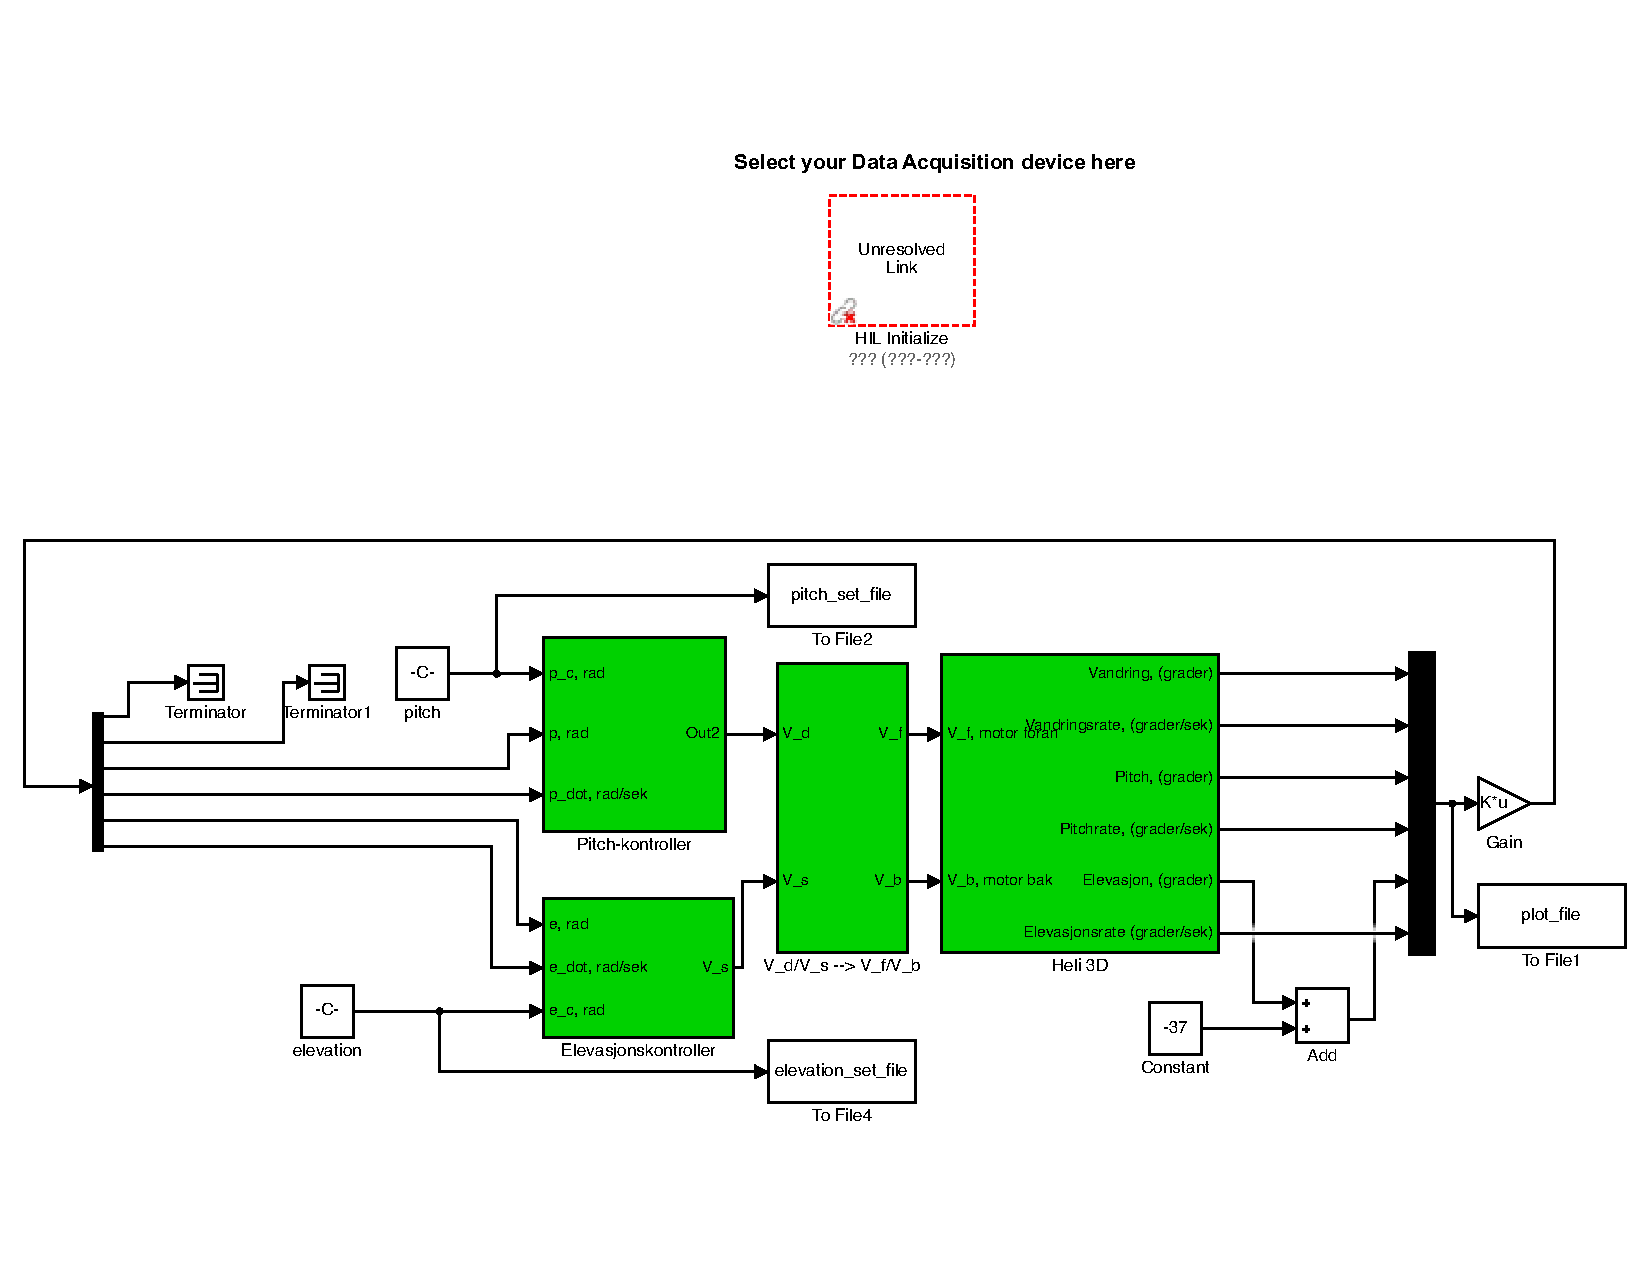
\includegraphics[width=1\textwidth]{helikoptertest}}
\caption{Simulink for test of helicopter}
\label{fig:testrunSim}
\end{figure}

\newpage
\subsection{Without feedback - Section \ref{sec:prob2}}\label{sec:simulink:2}
Figure~\ref{fig:without} shows a Simulink diagram for optimal control of pitch and travel without feedback.


\begin{figure}[!h]
\centerline{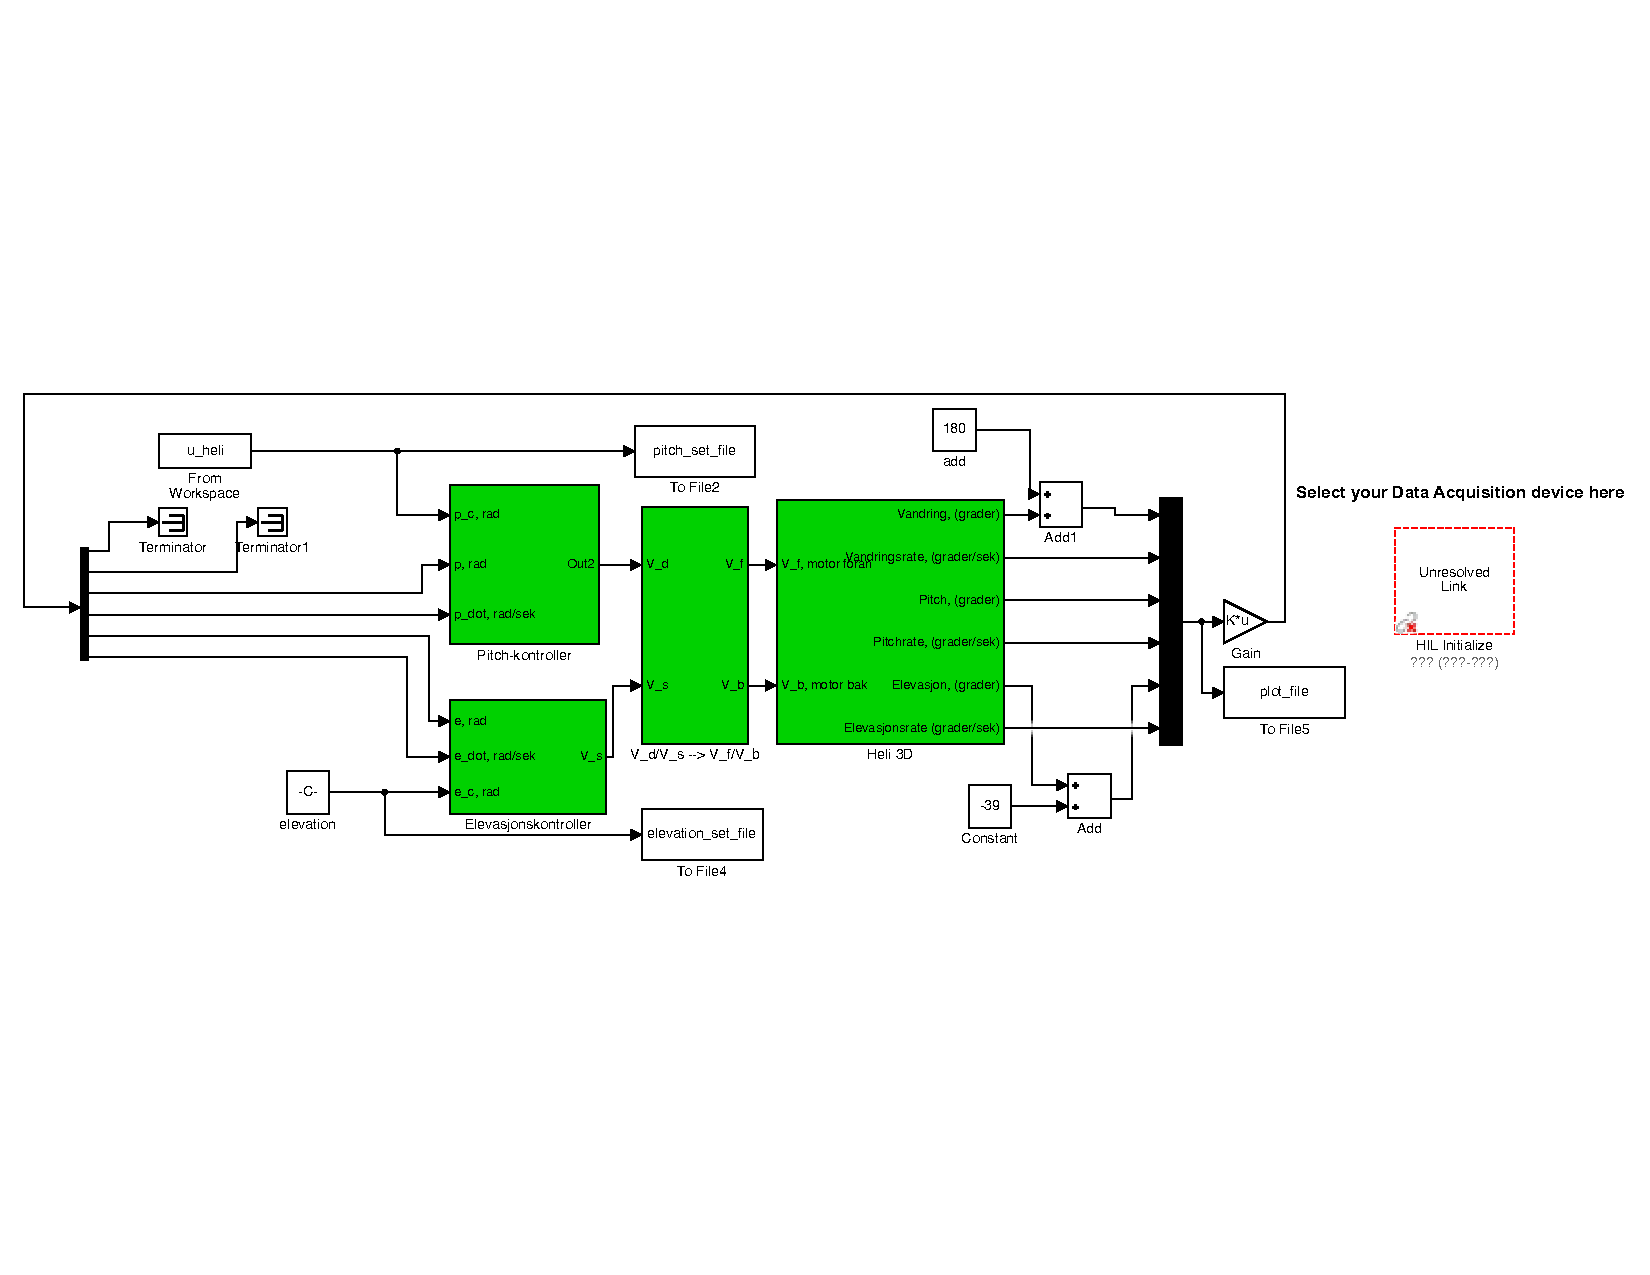
\includegraphics[width=1\textwidth]{helikopter10_2_without_feed}}
\caption{Optimal control of pitch and travel without feedback}
\label{fig:without}
\end{figure}

\newpage
\subsection{With feedback - Section \ref{sec:prob3}}\label{sec:simulink:3}
Figure~\ref{fig:with} shows a Simulink diagram for the initial setup of the helicopter.


\begin{figure}[!h]
\centerline{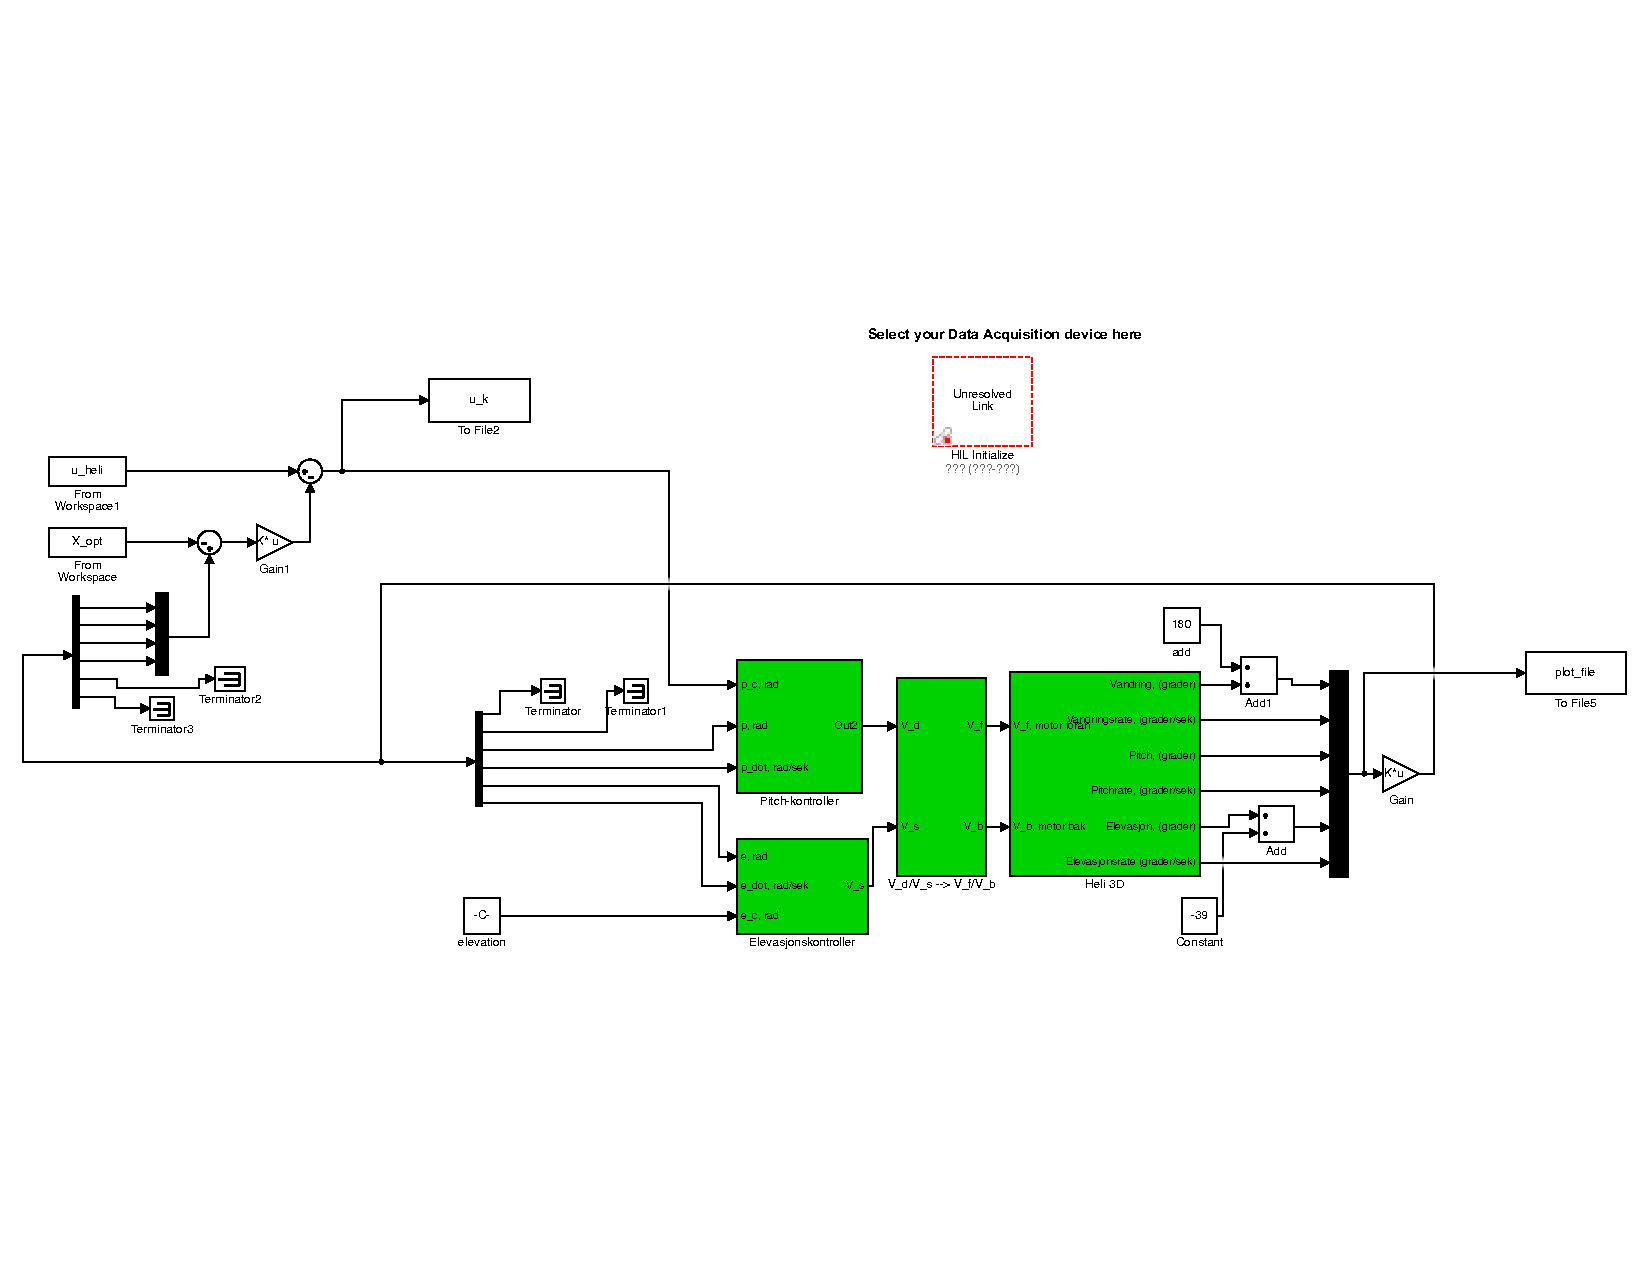
\includegraphics[width=1\textwidth]{helikopter10_3_2}}
\caption{Optimal control of pitch and travel with feedback}
\label{fig:with}
\end{figure}

\begin{figure}[htb]
	\centering
		%\includegraphics[width = \textwidth]{figures/simulink.pdf}
	\caption{A Simulink diagram.}
	\label{fig:simulink}
\end{figure}

\clearpage
\bibliographystyle{apalike}
\bibliography{helibib}\label{sec:bibliography}


\end{document}